\documentclass[1p]{elsarticle_modified}
%\bibliographystyle{elsarticle-num}

%\usepackage[colorlinks]{hyperref}
%\usepackage{abbrmath_seonhwa} %\Abb, \Ascr, \Acal ,\Abf, \Afrak
\usepackage{amsfonts}
\usepackage{amssymb}
\usepackage{amsmath}
\usepackage{amsthm}
\usepackage{scalefnt}
\usepackage{amsbsy}
\usepackage{kotex}
\usepackage{caption}
\usepackage{subfig}
\usepackage{color}
\usepackage{graphicx}
\usepackage{xcolor} %% white, black, red, green, blue, cyan, magenta, yellow
\usepackage{float}
\usepackage{setspace}
\usepackage{hyperref}

\usepackage{tikz}
\usetikzlibrary{arrows}

\usepackage{multirow}
\usepackage{array} % fixed length table
\usepackage{hhline}

%%%%%%%%%%%%%%%%%%%%%
\makeatletter
\renewcommand*\env@matrix[1][\arraystretch]{%
	\edef\arraystretch{#1}%
	\hskip -\arraycolsep
	\let\@ifnextchar\new@ifnextchar
	\array{*\c@MaxMatrixCols c}}
\makeatother %https://tex.stackexchange.com/questions/14071/how-can-i-increase-the-line-spacing-in-a-matrix
%%%%%%%%%%%%%%%

\usepackage[normalem]{ulem}

\newcommand{\msout}[1]{\ifmmode\text{\sout{\ensuremath{#1}}}\else\sout{#1}\fi}
%SOURCE: \msout is \stkout macro in https://tex.stackexchange.com/questions/20609/strikeout-in-math-mode

\newcommand{\cancel}[1]{
	\ifmmode
	{\color{red}\msout{#1}}
	\else
	{\color{red}\sout{#1}}
	\fi
}

\newcommand{\add}[1]{
	{\color{blue}\uwave{#1}}
}

\newcommand{\replace}[2]{
	\ifmmode
	{\color{red}\msout{#1}}{\color{blue}\uwave{#2}}
	\else
	{\color{red}\sout{#1}}{\color{blue}\uwave{#2}}
	\fi
}

\newcommand{\Sol}{\mathcal{S}} %segment
\newcommand{\D}{D} %diagram
\newcommand{\A}{\mathcal{A}} %arc


%%%%%%%%%%%%%%%%%%%%%%%%%%%%%5 test

\def\sl{\operatorname{\textup{SL}}(2,\Cbb)}
\def\psl{\operatorname{\textup{PSL}}(2,\Cbb)}
\def\quan{\mkern 1mu \triangleright \mkern 1mu}

\theoremstyle{definition}
\newtheorem{thm}{Theorem}[section]
\newtheorem{prop}[thm]{Proposition}
\newtheorem{lem}[thm]{Lemma}
\newtheorem{ques}[thm]{Question}
\newtheorem{cor}[thm]{Corollary}
\newtheorem{defn}[thm]{Definition}
\newtheorem{exam}[thm]{Example}
\newtheorem{rmk}[thm]{Remark}
\newtheorem{alg}[thm]{Algorithm}

\newcommand{\I}{\sqrt{-1}}
\begin{document}

%\begin{frontmatter}
%
%\title{Boundary parabolic representations of knots up to 8 crossings}
%
%%% Group authors per affiliation:
%\author{Yunhi Cho} 
%\address{Department of Mathematics, University of Seoul, Seoul, Korea}
%\ead{yhcho@uos.ac.kr}
%
%
%\author{Seonhwa Kim} %\fnref{s_kim}}
%\address{Center for Geometry and Physics, Institute for Basic Science, Pohang, 37673, Korea}
%\ead{ryeona17@ibs.re.kr}
%
%\author{Hyuk Kim}
%\address{Department of Mathematical Sciences, Seoul National University, Seoul 08826, Korea}
%\ead{hyukkim@snu.ac.kr}
%
%\author{Seokbeom Yoon}
%\address{Department of Mathematical Sciences, Seoul National University, Seoul, 08826,  Korea}
%\ead{sbyoon15@snu.ac.kr}
%
%\begin{abstract}
%We find all boundary parabolic representation of knots up to 8 crossings.
%
%\end{abstract}
%\begin{keyword}
%    \MSC[2010] 57M25 
%\end{keyword}
%
%\end{frontmatter}

%\linenumbers
%\tableofcontents
%
\newcommand\colored[1]{\textcolor{white}{\rule[-0.35ex]{0.8em}{1.4ex}}\kern-0.8em\color{red} #1}%
%\newcommand\colored[1]{\textcolor{white}{ #1}\kern-2.17ex	\textcolor{white}{ #1}\kern-1.81ex	\textcolor{white}{ #1}\kern-2.15ex\color{red}#1	}

{\Large $\underline{12a_{0337}~(K12a_{0337})}$}

\setlength{\tabcolsep}{10pt}
\renewcommand{\arraystretch}{1.6}
\vspace{1cm}\begin{tabular}{m{100pt}>{\centering\arraybackslash}m{274pt}}
\multirow{5}{120pt}{
	\centering
	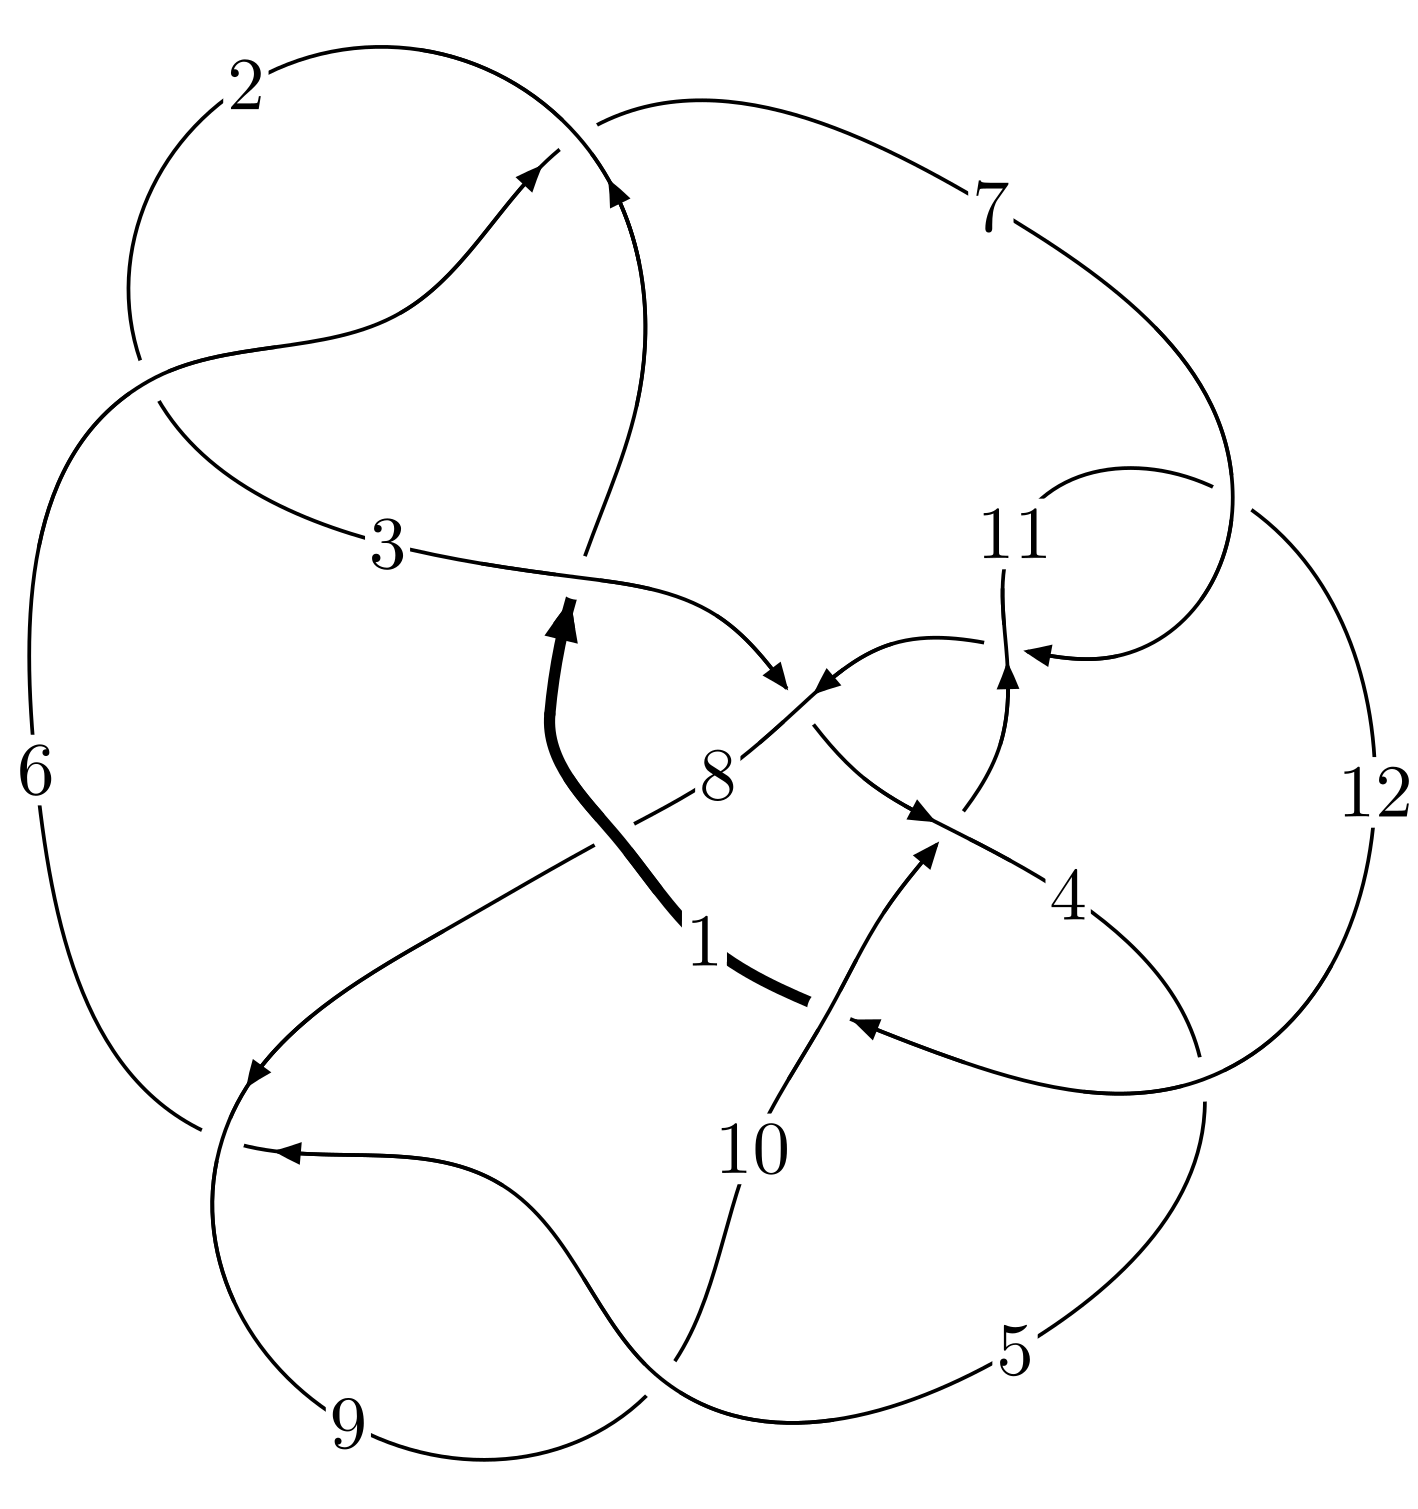
\includegraphics[width=112pt]{../../../GIT/diagram.site/Diagrams/png/1138_12a_0337.png}\\
\ \ \ A knot diagram\footnotemark}&
\allowdisplaybreaks
\textbf{Linearized knot diagam} \\
\cline{2-2}
 &
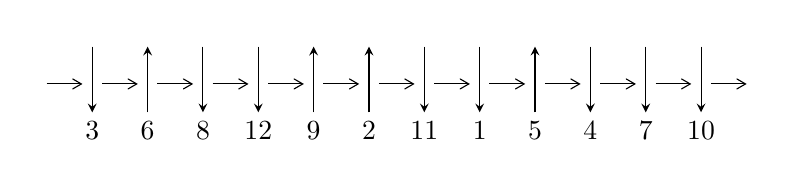
\begin{tikzpicture}[x=20pt, y=17pt]
	% nodes
	\node (C0) at (0, 0) {};
	\node (C1) at (1, 0) {};
	\node (C1U) at (1, +1) {};
	\node (C1D) at (1, -1) {3};

	\node (C2) at (2, 0) {};
	\node (C2U) at (2, +1) {};
	\node (C2D) at (2, -1) {6};

	\node (C3) at (3, 0) {};
	\node (C3U) at (3, +1) {};
	\node (C3D) at (3, -1) {8};

	\node (C4) at (4, 0) {};
	\node (C4U) at (4, +1) {};
	\node (C4D) at (4, -1) {12};

	\node (C5) at (5, 0) {};
	\node (C5U) at (5, +1) {};
	\node (C5D) at (5, -1) {9};

	\node (C6) at (6, 0) {};
	\node (C6U) at (6, +1) {};
	\node (C6D) at (6, -1) {2};

	\node (C7) at (7, 0) {};
	\node (C7U) at (7, +1) {};
	\node (C7D) at (7, -1) {11};

	\node (C8) at (8, 0) {};
	\node (C8U) at (8, +1) {};
	\node (C8D) at (8, -1) {1};

	\node (C9) at (9, 0) {};
	\node (C9U) at (9, +1) {};
	\node (C9D) at (9, -1) {5};

	\node (C10) at (10, 0) {};
	\node (C10U) at (10, +1) {};
	\node (C10D) at (10, -1) {4};

	\node (C11) at (11, 0) {};
	\node (C11U) at (11, +1) {};
	\node (C11D) at (11, -1) {7};

	\node (C12) at (12, 0) {};
	\node (C12U) at (12, +1) {};
	\node (C12D) at (12, -1) {10};
	\node (C13) at (13, 0) {};

	% arrows
	\draw[->,>={angle 60}]
	(C0) edge (C1) (C1) edge (C2) (C2) edge (C3) (C3) edge (C4) (C4) edge (C5) (C5) edge (C6) (C6) edge (C7) (C7) edge (C8) (C8) edge (C9) (C9) edge (C10) (C10) edge (C11) (C11) edge (C12) (C12) edge (C13) ;	\draw[->,>=stealth]
	(C1U) edge (C1D) (C2D) edge (C2U) (C3U) edge (C3D) (C4U) edge (C4D) (C5D) edge (C5U) (C6D) edge (C6U) (C7U) edge (C7D) (C8U) edge (C8D) (C9D) edge (C9U) (C10U) edge (C10D) (C11U) edge (C11D) (C12U) edge (C12D) ;
	\end{tikzpicture} \\
\hhline{~~} \\& 
\textbf{Solving Sequence} \\ \cline{2-2} 
 &
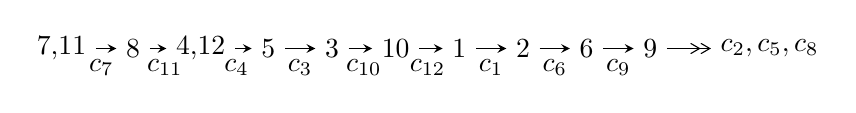
\begin{tikzpicture}[x=23pt, y=7pt]
	% node
	\node (A0) at (-1/8, 0) {7,11};
	\node (A1) at (1, 0) {8};
	\node (A2) at (33/16, 0) {4,12};
	\node (A3) at (25/8, 0) {5};
	\node (A4) at (33/8, 0) {3};
	\node (A5) at (41/8, 0) {10};
	\node (A6) at (49/8, 0) {1};
	\node (A7) at (57/8, 0) {2};
	\node (A8) at (65/8, 0) {6};
	\node (A9) at (73/8, 0) {9};
	\node (C1) at (1/2, -1) {$c_{7}$};
	\node (C2) at (3/2, -1) {$c_{11}$};
	\node (C3) at (21/8, -1) {$c_{4}$};
	\node (C4) at (29/8, -1) {$c_{3}$};
	\node (C5) at (37/8, -1) {$c_{10}$};
	\node (C6) at (45/8, -1) {$c_{12}$};
	\node (C7) at (53/8, -1) {$c_{1}$};
	\node (C8) at (61/8, -1) {$c_{6}$};
	\node (C9) at (69/8, -1) {$c_{9}$};
	\node (A10) at (11, 0) {$c_{2},c_{5},c_{8}$};

	% edge
	\draw[->,>=stealth]	
	(A0) edge (A1) (A1) edge (A2) (A2) edge (A3) (A3) edge (A4) (A4) edge (A5) (A5) edge (A6) (A6) edge (A7) (A7) edge (A8) (A8) edge (A9) ;
	\draw[->>,>={angle 60}]	
	(A9) edge (A10);
\end{tikzpicture} \\ 

\end{tabular} \\

\footnotetext{
The image of knot diagram is generated by the software ``\textbf{Draw programme}" developed by Andrew Bartholomew(\url{http://www.layer8.co.uk/maths/draw/index.htm\#Running-draw}), where we modified some parts for our purpose(\url{https://github.com/CATsTAILs/LinksPainter}).
}\phantom \\ \newline 
\centering \textbf{Ideals for irreducible components\footnotemark of $X_{\text{par}}$} 
 
\begin{align*}
I^u_{1}&=\langle 
3.92593\times10^{1072} u^{168}-9.52356\times10^{1071} u^{167}+\cdots+4.19834\times10^{1074} b-8.86904\times10^{1076},\\
\phantom{I^u_{1}}&\phantom{= \langle  }-2.28852\times10^{1076} u^{168}-4.03439\times10^{1075} u^{167}+\cdots+8.24512\times10^{1078} a+7.56272\times10^{1080},\\
\phantom{I^u_{1}}&\phantom{= \langle  }u^{169}- u^{168}+\cdots-396102 u-19639\rangle \\
I^u_{2}&=\langle 
-5.26255\times10^{26} u^{39}-1.81471\times10^{27} u^{38}+\cdots+2.28462\times10^{25} b+8.10299\times10^{26},\\
\phantom{I^u_{2}}&\phantom{= \langle  }-1.63791\times10^{27} u^{39}-6.96735\times10^{27} u^{38}+\cdots+2.28462\times10^{25} a-9.46245\times10^{26},\;u^{40}+4 u^{39}+\cdots-3 u+1\rangle \\
\\
\end{align*}
\raggedright * 2 irreducible components of $\dim_{\mathbb{C}}=0$, with total 209 representations.\\
\footnotetext{All coefficients of polynomials are rational numbers. But the coefficients are sometimes approximated in decimal forms when there is not enough margin.}
\newpage
\renewcommand{\arraystretch}{1}
\centering \section*{I. $I^u_{1}= \langle 3.93\times10^{1072} u^{168}-9.52\times10^{1071} u^{167}+\cdots+4.20\times10^{1074} b-8.87\times10^{1076},\;-2.29\times10^{1076} u^{168}-4.03\times10^{1075} u^{167}+\cdots+8.25\times10^{1078} a+7.56\times10^{1080},\;u^{169}- u^{168}+\cdots-396102 u-19639 \rangle$}
\flushleft \textbf{(i) Arc colorings}\\
\begin{tabular}{m{7pt} m{180pt} m{7pt} m{180pt} }
\flushright $a_{7}=$&$\begin{pmatrix}1\\0\end{pmatrix}$ \\
\flushright $a_{11}=$&$\begin{pmatrix}0\\u\end{pmatrix}$ \\
\flushright $a_{8}=$&$\begin{pmatrix}1\\u^2\end{pmatrix}$ \\
\flushright $a_{4}=$&$\begin{pmatrix}0.00277560 u^{168}+0.000489306 u^{167}+\cdots-1770.17 u-91.7235\\-0.00935115 u^{168}+0.00226841 u^{167}+\cdots+4433.82 u+211.251\end{pmatrix}$ \\
\flushright $a_{12}=$&$\begin{pmatrix}- u\\u\end{pmatrix}$ \\
\flushright $a_{5}=$&$\begin{pmatrix}-0.00248672 u^{168}+0.00363328 u^{167}+\cdots-128.783 u-16.7451\\-0.00408883 u^{168}-0.000875564 u^{167}+\cdots+2792.44 u+136.272\end{pmatrix}$ \\
\flushright $a_{3}=$&$\begin{pmatrix}-0.00274440 u^{168}+0.000612743 u^{167}+\cdots+1315.91 u+55.4079\\-0.00423005 u^{168}+0.000818225 u^{167}+\cdots+2187.83 u+105.268\end{pmatrix}$ \\
\flushright $a_{10}=$&$\begin{pmatrix}-0.0141723 u^{168}+0.00354478 u^{167}+\cdots+7349.15 u+355.698\\0.0232313 u^{168}-0.0194908 u^{167}+\cdots-5114.51 u-230.461\end{pmatrix}$ \\
\flushright $a_{1}=$&$\begin{pmatrix}0.0149427 u^{168}+0.0204386 u^{167}+\cdots-19447.8 u-966.256\\-0.0280194 u^{168}+0.0124714 u^{167}+\cdots+11581.6 u+549.700\end{pmatrix}$ \\
\flushright $a_{2}=$&$\begin{pmatrix}-0.0195512 u^{168}+0.0521669 u^{167}+\cdots-13686.9 u-715.490\\-0.00373791 u^{168}-0.00854166 u^{167}+\cdots+6735.90 u+334.898\end{pmatrix}$ \\
\flushright $a_{6}=$&$\begin{pmatrix}0.00324757 u^{168}+0.0252228 u^{167}+\cdots-14948.1 u-750.981\\0.00709202 u^{168}-0.0161873 u^{167}+\cdots+3582.84 u+189.182\end{pmatrix}$ \\
\flushright $a_{9}=$&$\begin{pmatrix}0.0348428 u^{168}-0.0745046 u^{167}+\cdots+15120.9 u+809.421\\-0.000778314 u^{168}+0.0204357 u^{167}+\cdots-9398.65 u-477.367\end{pmatrix}$\\&\end{tabular}
\flushleft \textbf{(ii) Obstruction class $= -1$}\\~\\
\flushleft \textbf{(iii) Cusp Shapes $= -0.0562127 u^{168}+0.0360147 u^{167}+\cdots+18248.3 u+848.574$}\\~\\
\newpage\renewcommand{\arraystretch}{1}
\flushleft \textbf{(iv) u-Polynomials at the component}\newline \\
\begin{tabular}{m{50pt}|m{274pt}}
Crossings & \hspace{64pt}u-Polynomials at each crossing \\
\hline $$\begin{aligned}c_{1}\end{aligned}$$&$\begin{aligned}
&u^{169}+82 u^{168}+\cdots-2175796 u-290521
\end{aligned}$\\
\hline $$\begin{aligned}c_{2},c_{6}\end{aligned}$$&$\begin{aligned}
&u^{169}+41 u^{167}+\cdots+3738 u+539
\end{aligned}$\\
\hline $$\begin{aligned}c_{3}\end{aligned}$$&$\begin{aligned}
&u^{169}-3 u^{168}+\cdots+179265310 u+1814710771
\end{aligned}$\\
\hline $$\begin{aligned}c_{4}\end{aligned}$$&$\begin{aligned}
&u^{169}+5 u^{168}+\cdots-536700 u+54209
\end{aligned}$\\
\hline $$\begin{aligned}c_{5},c_{9}\end{aligned}$$&$\begin{aligned}
&u^{169}-4 u^{168}+\cdots-251625 u+225625
\end{aligned}$\\
\hline $$\begin{aligned}c_{7},c_{11}\end{aligned}$$&$\begin{aligned}
&u^{169}+u^{168}+\cdots-396102 u+19639
\end{aligned}$\\
\hline $$\begin{aligned}c_{8}\end{aligned}$$&$\begin{aligned}
&u^{169}+3 u^{168}+\cdots-5120400 u+678325
\end{aligned}$\\
\hline $$\begin{aligned}c_{10}\end{aligned}$$&$\begin{aligned}
&u^{169}-2 u^{168}+\cdots+16242719 u+2056633
\end{aligned}$\\
\hline $$\begin{aligned}c_{12}\end{aligned}$$&$\begin{aligned}
&u^{169}-15 u^{168}+\cdots-22 u+1
\end{aligned}$\\
\hline
\end{tabular}\\~\\
\newpage\renewcommand{\arraystretch}{1}
\flushleft \textbf{(v) Riley Polynomials at the component}\newline \\
\begin{tabular}{m{50pt}|m{274pt}}
Crossings & \hspace{64pt}Riley Polynomials at each crossing \\
\hline $$\begin{aligned}c_{1}\end{aligned}$$&$\begin{aligned}
&y^{169}+30 y^{168}+\cdots+30317871838072 y-84402451441
\end{aligned}$\\
\hline $$\begin{aligned}c_{2},c_{6}\end{aligned}$$&$\begin{aligned}
&y^{169}+82 y^{168}+\cdots-2175796 y-290521
\end{aligned}$\\
\hline $$\begin{aligned}c_{3}\end{aligned}$$&$\begin{aligned}
&y^{169}+49 y^{168}+\cdots-1.47\times10^{20} y-3.29\times10^{18}
\end{aligned}$\\
\hline $$\begin{aligned}c_{4}\end{aligned}$$&$\begin{aligned}
&y^{169}-25 y^{168}+\cdots+99052632400 y-2938615681
\end{aligned}$\\
\hline $$\begin{aligned}c_{5},c_{9}\end{aligned}$$&$\begin{aligned}
&y^{169}+110 y^{168}+\cdots-2073635640625 y-50906640625
\end{aligned}$\\
\hline $$\begin{aligned}c_{7},c_{11}\end{aligned}$$&$\begin{aligned}
&y^{169}+99 y^{168}+\cdots-26158246040 y-385690321
\end{aligned}$\\
\hline $$\begin{aligned}c_{8}\end{aligned}$$&$\begin{aligned}
&y^{169}-11 y^{168}+\cdots-7757553615350 y-460124805625
\end{aligned}$\\
\hline $$\begin{aligned}c_{10}\end{aligned}$$&$\begin{aligned}
&y^{169}+28 y^{168}+\cdots-311436565903035 y-4229739296689
\end{aligned}$\\
\hline $$\begin{aligned}c_{12}\end{aligned}$$&$\begin{aligned}
&y^{169}-31 y^{168}+\cdots-68 y-1
\end{aligned}$\\
\hline
\end{tabular}\\~\\
\newpage\flushleft \textbf{(vi) Complex Volumes and Cusp Shapes}
$$\begin{array}{c|c|c}  
\text{Solutions to }I^u_{1}& \I (\text{vol} + \sqrt{-1}CS) & \text{Cusp shape}\\
 \hline 
\begin{aligned}
u &= \phantom{-}0.044658 + 1.006500 I \\
a &= \phantom{-}0.996465 + 0.535032 I \\
b &= -1.43140 + 0.97912 I\end{aligned}
 & \phantom{-}4.07610 - 0.13098 I & \phantom{-0.000000 } 0 \\ \hline\begin{aligned}
u &= \phantom{-}0.044658 - 1.006500 I \\
a &= \phantom{-}0.996465 - 0.535032 I \\
b &= -1.43140 - 0.97912 I\end{aligned}
 & \phantom{-}4.07610 + 0.13098 I & \phantom{-0.000000 } 0 \\ \hline\begin{aligned}
u &= -0.396532 + 0.907773 I \\
a &= -0.879383 - 0.331628 I \\
b &= \phantom{-}2.45190 + 1.07462 I\end{aligned}
 & -3.76122 + 10.95180 I & \phantom{-0.000000 } 0 \\ \hline\begin{aligned}
u &= -0.396532 - 0.907773 I \\
a &= -0.879383 + 0.331628 I \\
b &= \phantom{-}2.45190 - 1.07462 I\end{aligned}
 & -3.76122 - 10.95180 I & \phantom{-0.000000 } 0 \\ \hline\begin{aligned}
u &= -0.981868 + 0.268384 I \\
a &= -0.536866 - 0.625015 I \\
b &= -0.139872 - 0.451873 I\end{aligned}
 & -3.21924 - 1.51303 I & \phantom{-0.000000 } 0 \\ \hline\begin{aligned}
u &= -0.981868 - 0.268384 I \\
a &= -0.536866 + 0.625015 I \\
b &= -0.139872 + 0.451873 I\end{aligned}
 & -3.21924 + 1.51303 I & \phantom{-0.000000 } 0 \\ \hline\begin{aligned}
u &= -0.171939 + 0.966185 I \\
a &= -0.697577 - 0.328817 I \\
b &= \phantom{-}2.02253 + 1.39734 I\end{aligned}
 & -4.74972 + 3.36342 I & \phantom{-0.000000 } 0 \\ \hline\begin{aligned}
u &= -0.171939 - 0.966185 I \\
a &= -0.697577 + 0.328817 I \\
b &= \phantom{-}2.02253 - 1.39734 I\end{aligned}
 & -4.74972 - 3.36342 I & \phantom{-0.000000 } 0 \\ \hline\begin{aligned}
u &= \phantom{-}0.093339 + 0.971134 I \\
a &= \phantom{-}0.48303 - 1.78499 I \\
b &= -0.690468 + 0.841642 I\end{aligned}
 & \phantom{-}2.16298 + 1.20126 I & \phantom{-0.000000 } 0 \\ \hline\begin{aligned}
u &= \phantom{-}0.093339 - 0.971134 I \\
a &= \phantom{-}0.48303 + 1.78499 I \\
b &= -0.690468 - 0.841642 I\end{aligned}
 & \phantom{-}2.16298 - 1.20126 I & \phantom{-0.000000 } 0\\
 \hline 
 \end{array}$$\newpage$$\begin{array}{c|c|c}  
\text{Solutions to }I^u_{1}& \I (\text{vol} + \sqrt{-1}CS) & \text{Cusp shape}\\
 \hline 
\begin{aligned}
u &= -1.013160 + 0.152109 I \\
a &= -0.517938 - 1.096390 I \\
b &= -0.031377 + 0.201783 I\end{aligned}
 & \phantom{-}1.61645 - 8.36601 I & \phantom{-0.000000 } 0 \\ \hline\begin{aligned}
u &= -1.013160 - 0.152109 I \\
a &= -0.517938 + 1.096390 I \\
b &= -0.031377 - 0.201783 I\end{aligned}
 & \phantom{-}1.61645 + 8.36601 I & \phantom{-0.000000 } 0 \\ \hline\begin{aligned}
u &= \phantom{-}0.255344 + 0.994298 I \\
a &= -0.50826 + 1.76913 I \\
b &= \phantom{-}0.654381 - 0.952277 I\end{aligned}
 & \phantom{-}1.46223 - 4.10465 I & \phantom{-0.000000 } 0 \\ \hline\begin{aligned}
u &= \phantom{-}0.255344 - 0.994298 I \\
a &= -0.50826 - 1.76913 I \\
b &= \phantom{-}0.654381 + 0.952277 I\end{aligned}
 & \phantom{-}1.46223 + 4.10465 I & \phantom{-0.000000 } 0 \\ \hline\begin{aligned}
u &= \phantom{-}0.529439 + 0.880204 I \\
a &= -1.26930 + 2.16055 I \\
b &= \phantom{-}1.51032 - 1.75216 I\end{aligned}
 & -0.220436 - 0.346158 I & \phantom{-0.000000 } 0 \\ \hline\begin{aligned}
u &= \phantom{-}0.529439 - 0.880204 I \\
a &= -1.26930 - 2.16055 I \\
b &= \phantom{-}1.51032 + 1.75216 I\end{aligned}
 & -0.220436 + 0.346158 I & \phantom{-0.000000 } 0 \\ \hline\begin{aligned}
u &= \phantom{-}0.117310 + 1.021390 I \\
a &= -0.749632 + 0.443480 I \\
b &= \phantom{-}1.71239 - 0.64949 I\end{aligned}
 & \phantom{-}2.25549 - 1.65445 I & \phantom{-0.000000 } 0 \\ \hline\begin{aligned}
u &= \phantom{-}0.117310 - 1.021390 I \\
a &= -0.749632 - 0.443480 I \\
b &= \phantom{-}1.71239 + 0.64949 I\end{aligned}
 & \phantom{-}2.25549 + 1.65445 I & \phantom{-0.000000 } 0 \\ \hline\begin{aligned}
u &= -0.243111 + 1.006920 I \\
a &= \phantom{-}0.05471 - 1.87049 I \\
b &= -0.545638 + 0.917625 I\end{aligned}
 & -0.38728 + 5.60268 I & \phantom{-0.000000 } 0 \\ \hline\begin{aligned}
u &= -0.243111 - 1.006920 I \\
a &= \phantom{-}0.05471 + 1.87049 I \\
b &= -0.545638 - 0.917625 I\end{aligned}
 & -0.38728 - 5.60268 I & \phantom{-0.000000 } 0\\
 \hline 
 \end{array}$$\newpage$$\begin{array}{c|c|c}  
\text{Solutions to }I^u_{1}& \I (\text{vol} + \sqrt{-1}CS) & \text{Cusp shape}\\
 \hline 
\begin{aligned}
u &= \phantom{-}0.487958 + 0.822863 I \\
a &= \phantom{-}1.35922 + 0.44746 I \\
b &= -1.72022 - 0.45455 I\end{aligned}
 & -0.47180 - 3.31768 I & \phantom{-0.000000 } 0 \\ \hline\begin{aligned}
u &= \phantom{-}0.487958 - 0.822863 I \\
a &= \phantom{-}1.35922 - 0.44746 I \\
b &= -1.72022 + 0.45455 I\end{aligned}
 & -0.47180 + 3.31768 I & \phantom{-0.000000 } 0 \\ \hline\begin{aligned}
u &= \phantom{-}0.164962 + 1.030540 I \\
a &= -1.006610 - 0.788628 I \\
b &= \phantom{-}1.47748 - 0.73298 I\end{aligned}
 & \phantom{-}1.08617 - 5.18124 I & \phantom{-0.000000 } 0 \\ \hline\begin{aligned}
u &= \phantom{-}0.164962 - 1.030540 I \\
a &= -1.006610 + 0.788628 I \\
b &= \phantom{-}1.47748 + 0.73298 I\end{aligned}
 & \phantom{-}1.08617 + 5.18124 I & \phantom{-0.000000 } 0 \\ \hline\begin{aligned}
u &= \phantom{-}0.637612 + 0.827670 I \\
a &= \phantom{-}0.287707 + 0.683609 I \\
b &= -0.899194 - 0.137007 I\end{aligned}
 & -1.15857 - 2.50493 I & \phantom{-0.000000 } 0 \\ \hline\begin{aligned}
u &= \phantom{-}0.637612 - 0.827670 I \\
a &= \phantom{-}0.287707 - 0.683609 I \\
b &= -0.899194 + 0.137007 I\end{aligned}
 & -1.15857 + 2.50493 I & \phantom{-0.000000 } 0 \\ \hline\begin{aligned}
u &= \phantom{-}0.918343 + 0.499765 I \\
a &= -0.294949 + 0.622152 I \\
b &= -0.0997323 - 0.0246033 I\end{aligned}
 & -2.67503 - 1.97184 I & \phantom{-0.000000 } 0 \\ \hline\begin{aligned}
u &= \phantom{-}0.918343 - 0.499765 I \\
a &= -0.294949 - 0.622152 I \\
b &= -0.0997323 + 0.0246033 I\end{aligned}
 & -2.67503 + 1.97184 I & \phantom{-0.000000 } 0 \\ \hline\begin{aligned}
u &= \phantom{-}0.909378 + 0.180627 I \\
a &= \phantom{-}0.691868 - 1.066250 I \\
b &= \phantom{-}0.388140 + 0.094170 I\end{aligned}
 & -7.02483 + 5.88488 I & \phantom{-0.000000 } 0 \\ \hline\begin{aligned}
u &= \phantom{-}0.909378 - 0.180627 I \\
a &= \phantom{-}0.691868 + 1.066250 I \\
b &= \phantom{-}0.388140 - 0.094170 I\end{aligned}
 & -7.02483 - 5.88488 I & \phantom{-0.000000 } 0\\
 \hline 
 \end{array}$$\newpage$$\begin{array}{c|c|c}  
\text{Solutions to }I^u_{1}& \I (\text{vol} + \sqrt{-1}CS) & \text{Cusp shape}\\
 \hline 
\begin{aligned}
u &= \phantom{-}0.665089 + 0.841948 I \\
a &= -1.44303 - 0.65524 I \\
b &= \phantom{-}1.71644 + 0.47777 I\end{aligned}
 & -0.935542 - 0.093932 I & \phantom{-0.000000 } 0 \\ \hline\begin{aligned}
u &= \phantom{-}0.665089 - 0.841948 I \\
a &= -1.44303 + 0.65524 I \\
b &= \phantom{-}1.71644 - 0.47777 I\end{aligned}
 & -0.935542 + 0.093932 I & \phantom{-0.000000 } 0 \\ \hline\begin{aligned}
u &= \phantom{-}0.850717 + 0.353274 I \\
a &= -0.393947 - 0.813121 I \\
b &= \phantom{-}0.638918 - 0.558945 I\end{aligned}
 & -4.73336 + 0.52961 I & \phantom{-0.000000 } 0 \\ \hline\begin{aligned}
u &= \phantom{-}0.850717 - 0.353274 I \\
a &= -0.393947 + 0.813121 I \\
b &= \phantom{-}0.638918 + 0.558945 I\end{aligned}
 & -4.73336 - 0.52961 I & \phantom{-0.000000 } 0 \\ \hline\begin{aligned}
u &= -0.919592 + 0.049951 I \\
a &= \phantom{-}0.602634 + 1.089060 I \\
b &= \phantom{-}0.072369 - 0.282821 I\end{aligned}
 & \phantom{-}3.12409 - 3.25295 I & \phantom{-0.000000 } 0 \\ \hline\begin{aligned}
u &= -0.919592 - 0.049951 I \\
a &= \phantom{-}0.602634 - 1.089060 I \\
b &= \phantom{-}0.072369 + 0.282821 I\end{aligned}
 & \phantom{-}3.12409 + 3.25295 I & \phantom{-0.000000 } 0 \\ \hline\begin{aligned}
u &= \phantom{-}0.480150 + 0.784625 I \\
a &= \phantom{-}1.42087 - 1.31084 I \\
b &= -1.98518 + 0.98754 I\end{aligned}
 & -0.51792 - 3.83639 I & \phantom{-0.000000 } 0 \\ \hline\begin{aligned}
u &= \phantom{-}0.480150 - 0.784625 I \\
a &= \phantom{-}1.42087 + 1.31084 I \\
b &= -1.98518 - 0.98754 I\end{aligned}
 & -0.51792 + 3.83639 I & \phantom{-0.000000 } 0 \\ \hline\begin{aligned}
u &= \phantom{-}0.634756 + 0.660746 I \\
a &= \phantom{-}0.862405 + 0.649285 I \\
b &= -1.177500 + 0.152789 I\end{aligned}
 & -1.42111 - 2.39910 I & \phantom{-0.000000 } 0 \\ \hline\begin{aligned}
u &= \phantom{-}0.634756 - 0.660746 I \\
a &= \phantom{-}0.862405 - 0.649285 I \\
b &= -1.177500 - 0.152789 I\end{aligned}
 & -1.42111 + 2.39910 I & \phantom{-0.000000 } 0\\
 \hline 
 \end{array}$$\newpage$$\begin{array}{c|c|c}  
\text{Solutions to }I^u_{1}& \I (\text{vol} + \sqrt{-1}CS) & \text{Cusp shape}\\
 \hline 
\begin{aligned}
u &= -0.337055 + 1.033500 I \\
a &= \phantom{-}0.03805 + 1.73437 I \\
b &= \phantom{-}0.495058 - 0.843473 I\end{aligned}
 & -2.63977 + 11.53680 I & \phantom{-0.000000 } 0 \\ \hline\begin{aligned}
u &= -0.337055 - 1.033500 I \\
a &= \phantom{-}0.03805 - 1.73437 I \\
b &= \phantom{-}0.495058 + 0.843473 I\end{aligned}
 & -2.63977 - 11.53680 I & \phantom{-0.000000 } 0 \\ \hline\begin{aligned}
u &= \phantom{-}0.744470 + 0.802902 I \\
a &= \phantom{-}0.252829 - 0.637078 I \\
b &= \phantom{-}0.317423 - 0.123344 I\end{aligned}
 & -3.74753 + 0.87759 I & \phantom{-0.000000 } 0 \\ \hline\begin{aligned}
u &= \phantom{-}0.744470 - 0.802902 I \\
a &= \phantom{-}0.252829 + 0.637078 I \\
b &= \phantom{-}0.317423 + 0.123344 I\end{aligned}
 & -3.74753 - 0.87759 I & \phantom{-0.000000 } 0 \\ \hline\begin{aligned}
u &= -0.518056 + 0.739375 I \\
a &= \phantom{-}0.26197 + 1.47711 I \\
b &= -0.076528 + 0.214474 I\end{aligned}
 & -4.22824 - 7.18268 I & \phantom{-0.000000 } 0 \\ \hline\begin{aligned}
u &= -0.518056 - 0.739375 I \\
a &= \phantom{-}0.26197 - 1.47711 I \\
b &= -0.076528 - 0.214474 I\end{aligned}
 & -4.22824 + 7.18268 I & \phantom{-0.000000 } 0 \\ \hline\begin{aligned}
u &= -0.325716 + 1.051690 I \\
a &= -0.524341 - 0.026961 I \\
b &= \phantom{-}1.39349 - 0.97278 I\end{aligned}
 & \phantom{-}1.78089 - 0.06211 I & \phantom{-0.000000 } 0 \\ \hline\begin{aligned}
u &= -0.325716 - 1.051690 I \\
a &= -0.524341 + 0.026961 I \\
b &= \phantom{-}1.39349 + 0.97278 I\end{aligned}
 & \phantom{-}1.78089 + 0.06211 I & \phantom{-0.000000 } 0 \\ \hline\begin{aligned}
u &= -0.139866 + 0.883342 I \\
a &= -0.20598 + 2.41360 I \\
b &= \phantom{-}0.63697 - 1.28102 I\end{aligned}
 & -6.97912 + 1.85496 I & \phantom{-0.000000 } 0 \\ \hline\begin{aligned}
u &= -0.139866 - 0.883342 I \\
a &= -0.20598 - 2.41360 I \\
b &= \phantom{-}0.63697 + 1.28102 I\end{aligned}
 & -6.97912 - 1.85496 I & \phantom{-0.000000 } 0\\
 \hline 
 \end{array}$$\newpage$$\begin{array}{c|c|c}  
\text{Solutions to }I^u_{1}& \I (\text{vol} + \sqrt{-1}CS) & \text{Cusp shape}\\
 \hline 
\begin{aligned}
u &= -0.362552 + 1.052220 I \\
a &= \phantom{-}0.820612 + 0.232915 I \\
b &= -2.17809 - 0.99651 I\end{aligned}
 & -1.25299 + 6.67767 I & \phantom{-0.000000 } 0 \\ \hline\begin{aligned}
u &= -0.362552 - 1.052220 I \\
a &= \phantom{-}0.820612 - 0.232915 I \\
b &= -2.17809 + 0.99651 I\end{aligned}
 & -1.25299 - 6.67767 I & \phantom{-0.000000 } 0 \\ \hline\begin{aligned}
u &= -0.316884 + 0.827161 I \\
a &= -1.42786 - 0.54097 I \\
b &= \phantom{-}1.44083 + 1.13167 I\end{aligned}
 & -6.59870 + 0.31411 I & \phantom{-0.000000 } 0 \\ \hline\begin{aligned}
u &= -0.316884 - 0.827161 I \\
a &= -1.42786 + 0.54097 I \\
b &= \phantom{-}1.44083 - 1.13167 I\end{aligned}
 & -6.59870 - 0.31411 I & \phantom{-0.000000 } 0 \\ \hline\begin{aligned}
u &= \phantom{-}0.722812 + 0.849666 I \\
a &= -0.312481 - 0.251647 I \\
b &= \phantom{-}1.126120 - 0.443018 I\end{aligned}
 & -3.70060 - 6.37509 I & \phantom{-0.000000 } 0 \\ \hline\begin{aligned}
u &= \phantom{-}0.722812 - 0.849666 I \\
a &= -0.312481 + 0.251647 I \\
b &= \phantom{-}1.126120 + 0.443018 I\end{aligned}
 & -3.70060 + 6.37509 I & \phantom{-0.000000 } 0 \\ \hline\begin{aligned}
u &= -0.113414 + 0.863598 I \\
a &= -0.20814 + 1.50975 I \\
b &= -0.152741 + 0.235958 I\end{aligned}
 & -5.25151 - 1.93825 I & \phantom{-0.000000 } 0 \\ \hline\begin{aligned}
u &= -0.113414 - 0.863598 I \\
a &= -0.20814 - 1.50975 I \\
b &= -0.152741 - 0.235958 I\end{aligned}
 & -5.25151 + 1.93825 I & \phantom{-0.000000 } 0 \\ \hline\begin{aligned}
u &= \phantom{-}0.861467 + 0.732944 I \\
a &= -0.601544 - 0.457562 I \\
b &= \phantom{-}1.30603 - 0.54276 I\end{aligned}
 & -3.77410 - 6.48687 I & \phantom{-0.000000 } 0 \\ \hline\begin{aligned}
u &= \phantom{-}0.861467 - 0.732944 I \\
a &= -0.601544 + 0.457562 I \\
b &= \phantom{-}1.30603 + 0.54276 I\end{aligned}
 & -3.77410 + 6.48687 I & \phantom{-0.000000 } 0\\
 \hline 
 \end{array}$$\newpage$$\begin{array}{c|c|c}  
\text{Solutions to }I^u_{1}& \I (\text{vol} + \sqrt{-1}CS) & \text{Cusp shape}\\
 \hline 
\begin{aligned}
u &= -0.277299 + 0.815257 I \\
a &= \phantom{-}1.021070 - 0.012828 I \\
b &= -0.95184 + 1.20117 I\end{aligned}
 & \phantom{-}3.78329 + 1.09562 I & \phantom{-0.000000 } 0 \\ \hline\begin{aligned}
u &= -0.277299 - 0.815257 I \\
a &= \phantom{-}1.021070 + 0.012828 I \\
b &= -0.95184 - 1.20117 I\end{aligned}
 & \phantom{-}3.78329 - 1.09562 I & \phantom{-0.000000 } 0 \\ \hline\begin{aligned}
u &= \phantom{-}0.094182 + 0.843364 I \\
a &= -1.281380 - 0.429444 I \\
b &= \phantom{-}1.74284 - 1.24981 I\end{aligned}
 & \phantom{-}0.27541 + 3.96070 I & \phantom{-0.000000 } 0 \\ \hline\begin{aligned}
u &= \phantom{-}0.094182 - 0.843364 I \\
a &= -1.281380 + 0.429444 I \\
b &= \phantom{-}1.74284 + 1.24981 I\end{aligned}
 & \phantom{-}0.27541 - 3.96070 I & \phantom{-0.000000 } 0 \\ \hline\begin{aligned}
u &= \phantom{-}0.556157 + 1.017880 I \\
a &= \phantom{-}1.052950 - 0.039822 I \\
b &= -1.75925 + 0.32260 I\end{aligned}
 & -0.95403 - 3.29831 I & \phantom{-0.000000 } 0 \\ \hline\begin{aligned}
u &= \phantom{-}0.556157 - 1.017880 I \\
a &= \phantom{-}1.052950 + 0.039822 I \\
b &= -1.75925 - 0.32260 I\end{aligned}
 & -0.95403 + 3.29831 I & \phantom{-0.000000 } 0 \\ \hline\begin{aligned}
u &= -0.128532 + 1.158210 I \\
a &= \phantom{-}0.735181 - 0.664534 I \\
b &= -1.54167 - 0.44711 I\end{aligned}
 & \phantom{-}2.89877 + 3.44612 I & \phantom{-0.000000 } 0 \\ \hline\begin{aligned}
u &= -0.128532 - 1.158210 I \\
a &= \phantom{-}0.735181 + 0.664534 I \\
b &= -1.54167 + 0.44711 I\end{aligned}
 & \phantom{-}2.89877 - 3.44612 I & \phantom{-0.000000 } 0 \\ \hline\begin{aligned}
u &= \phantom{-}0.191760 + 0.805520 I \\
a &= \phantom{-}0.59127 - 1.30945 I \\
b &= \phantom{-}0.190963 - 0.241863 I\end{aligned}
 & -5.12988 - 5.13411 I & \phantom{-0.000000 } 0 \\ \hline\begin{aligned}
u &= \phantom{-}0.191760 - 0.805520 I \\
a &= \phantom{-}0.59127 + 1.30945 I \\
b &= \phantom{-}0.190963 + 0.241863 I\end{aligned}
 & -5.12988 + 5.13411 I & \phantom{-0.000000 } 0\\
 \hline 
 \end{array}$$\newpage$$\begin{array}{c|c|c}  
\text{Solutions to }I^u_{1}& \I (\text{vol} + \sqrt{-1}CS) & \text{Cusp shape}\\
 \hline 
\begin{aligned}
u &= \phantom{-}0.528840 + 1.047660 I \\
a &= \phantom{-}1.36975 + 0.63166 I \\
b &= -1.68830 - 0.46136 I\end{aligned}
 & \phantom{-}0.423917 - 0.974746 I & \phantom{-0.000000 } 0 \\ \hline\begin{aligned}
u &= \phantom{-}0.528840 - 1.047660 I \\
a &= \phantom{-}1.36975 - 0.63166 I \\
b &= -1.68830 + 0.46136 I\end{aligned}
 & \phantom{-}0.423917 + 0.974746 I & \phantom{-0.000000 } 0 \\ \hline\begin{aligned}
u &= \phantom{-}0.383343 + 1.112420 I \\
a &= \phantom{-}0.869750 + 0.003265 I \\
b &= -1.83620 - 0.31470 I\end{aligned}
 & -0.61499 - 3.61164 I & \phantom{-0.000000 } 0 \\ \hline\begin{aligned}
u &= \phantom{-}0.383343 - 1.112420 I \\
a &= \phantom{-}0.869750 - 0.003265 I \\
b &= -1.83620 + 0.31470 I\end{aligned}
 & -0.61499 + 3.61164 I & \phantom{-0.000000 } 0 \\ \hline\begin{aligned}
u &= -0.207338 + 1.164470 I \\
a &= \phantom{-}0.632980 + 0.316638 I \\
b &= -1.22898 + 1.05563 I\end{aligned}
 & \phantom{-}5.46852 + 1.26241 I & \phantom{-0.000000 } 0 \\ \hline\begin{aligned}
u &= -0.207338 - 1.164470 I \\
a &= \phantom{-}0.632980 - 0.316638 I \\
b &= -1.22898 - 1.05563 I\end{aligned}
 & \phantom{-}5.46852 - 1.26241 I & \phantom{-0.000000 } 0 \\ \hline\begin{aligned}
u &= -0.482216 + 1.114650 I \\
a &= \phantom{-}1.307440 + 0.079070 I \\
b &= -2.20536 - 0.60713 I\end{aligned}
 & \phantom{-}0.46009 + 6.79623 I & \phantom{-0.000000 } 0 \\ \hline\begin{aligned}
u &= -0.482216 - 1.114650 I \\
a &= \phantom{-}1.307440 - 0.079070 I \\
b &= -2.20536 + 0.60713 I\end{aligned}
 & \phantom{-}0.46009 - 6.79623 I & \phantom{-0.000000 } 0 \\ \hline\begin{aligned}
u &= \phantom{-}0.644814 + 1.035320 I \\
a &= -1.37569 - 0.65556 I \\
b &= \phantom{-}1.70413 + 0.46411 I\end{aligned}
 & -0.30092 - 5.14241 I & \phantom{-0.000000 } 0 \\ \hline\begin{aligned}
u &= \phantom{-}0.644814 - 1.035320 I \\
a &= -1.37569 + 0.65556 I \\
b &= \phantom{-}1.70413 - 0.46411 I\end{aligned}
 & -0.30092 + 5.14241 I & \phantom{-0.000000 } 0\\
 \hline 
 \end{array}$$\newpage$$\begin{array}{c|c|c}  
\text{Solutions to }I^u_{1}& \I (\text{vol} + \sqrt{-1}CS) & \text{Cusp shape}\\
 \hline 
\begin{aligned}
u &= \phantom{-}0.018602 + 1.222640 I \\
a &= -0.765291 + 0.453535 I \\
b &= \phantom{-}1.71467 + 0.50154 I\end{aligned}
 & \phantom{-}4.73347 - 1.96451 I & \phantom{-0.000000 } 0 \\ \hline\begin{aligned}
u &= \phantom{-}0.018602 - 1.222640 I \\
a &= -0.765291 - 0.453535 I \\
b &= \phantom{-}1.71467 - 0.50154 I\end{aligned}
 & \phantom{-}4.73347 + 1.96451 I & \phantom{-0.000000 } 0 \\ \hline\begin{aligned}
u &= -0.587870 + 0.505579 I \\
a &= -0.58178 - 1.44431 I \\
b &= \phantom{-}0.003890 - 0.265746 I\end{aligned}
 & -2.98450 - 2.85543 I & \phantom{-0.000000 } 0 \\ \hline\begin{aligned}
u &= -0.587870 - 0.505579 I \\
a &= -0.58178 + 1.44431 I \\
b &= \phantom{-}0.003890 + 0.265746 I\end{aligned}
 & -2.98450 + 2.85543 I & \phantom{-0.000000 } 0 \\ \hline\begin{aligned}
u &= -0.209643 + 1.206600 I \\
a &= \phantom{-}1.50917 + 0.38301 I \\
b &= -2.03434 - 0.73278 I\end{aligned}
 & \phantom{-}4.70660 - 1.76368 I & \phantom{-0.000000 } 0 \\ \hline\begin{aligned}
u &= -0.209643 - 1.206600 I \\
a &= \phantom{-}1.50917 - 0.38301 I \\
b &= -2.03434 + 0.73278 I\end{aligned}
 & \phantom{-}4.70660 + 1.76368 I & \phantom{-0.000000 } 0 \\ \hline\begin{aligned}
u &= -0.686146 + 0.340725 I \\
a &= -0.445255 - 1.340220 I \\
b &= -0.310313 + 0.072750 I\end{aligned}
 & -1.86442 - 2.29085 I & \phantom{-0.000000 } 0 \\ \hline\begin{aligned}
u &= -0.686146 - 0.340725 I \\
a &= -0.445255 + 1.340220 I \\
b &= -0.310313 - 0.072750 I\end{aligned}
 & -1.86442 + 2.29085 I & \phantom{-0.000000 } 0 \\ \hline\begin{aligned}
u &= \phantom{-}1.226690 + 0.147268 I \\
a &= -0.410408 + 0.826608 I \\
b &= -0.300675 + 0.005803 I\end{aligned}
 & -1.19680 + 8.26372 I & \phantom{-0.000000 } 0 \\ \hline\begin{aligned}
u &= \phantom{-}1.226690 - 0.147268 I \\
a &= -0.410408 - 0.826608 I \\
b &= -0.300675 - 0.005803 I\end{aligned}
 & -1.19680 - 8.26372 I & \phantom{-0.000000 } 0\\
 \hline 
 \end{array}$$\newpage$$\begin{array}{c|c|c}  
\text{Solutions to }I^u_{1}& \I (\text{vol} + \sqrt{-1}CS) & \text{Cusp shape}\\
 \hline 
\begin{aligned}
u &= -0.293350 + 1.207820 I \\
a &= -0.525166 - 0.288634 I \\
b &= \phantom{-}1.24314 - 1.11002 I\end{aligned}
 & \phantom{-}3.96218 + 6.03076 I & \phantom{-0.000000 } 0 \\ \hline\begin{aligned}
u &= -0.293350 - 1.207820 I \\
a &= -0.525166 + 0.288634 I \\
b &= \phantom{-}1.24314 + 1.11002 I\end{aligned}
 & \phantom{-}3.96218 - 6.03076 I & \phantom{-0.000000 } 0 \\ \hline\begin{aligned}
u &= -0.665318 + 0.343719 I \\
a &= \phantom{-}1.25428 + 0.69189 I \\
b &= \phantom{-}0.082099 - 0.574218 I\end{aligned}
 & -8.19155 + 2.92580 I & \phantom{-0.000000 } 0 \\ \hline\begin{aligned}
u &= -0.665318 - 0.343719 I \\
a &= \phantom{-}1.25428 - 0.69189 I \\
b &= \phantom{-}0.082099 + 0.574218 I\end{aligned}
 & -8.19155 - 2.92580 I & \phantom{-0.000000 } 0 \\ \hline\begin{aligned}
u &= -0.318853 + 1.226120 I \\
a &= -1.44155 - 0.27889 I \\
b &= \phantom{-}2.10623 + 0.65335 I\end{aligned}
 & \phantom{-}6.55505 + 4.24519 I & \phantom{-0.000000 } 0 \\ \hline\begin{aligned}
u &= -0.318853 - 1.226120 I \\
a &= -1.44155 + 0.27889 I \\
b &= \phantom{-}2.10623 - 0.65335 I\end{aligned}
 & \phantom{-}6.55505 - 4.24519 I & \phantom{-0.000000 } 0 \\ \hline\begin{aligned}
u &= -0.000042 + 0.728443 I \\
a &= \phantom{-}0.342818 - 0.698682 I \\
b &= -1.76952 + 0.79957 I\end{aligned}
 & \phantom{-}0.06361 + 2.18446 I & \phantom{-0.000000 } 0 \\ \hline\begin{aligned}
u &= -0.000042 - 0.728443 I \\
a &= \phantom{-}0.342818 + 0.698682 I \\
b &= -1.76952 - 0.79957 I\end{aligned}
 & \phantom{-}0.06361 - 2.18446 I & \phantom{-0.000000 } 0 \\ \hline\begin{aligned}
u &= \phantom{-}1.255590 + 0.254380 I \\
a &= \phantom{-}0.346889 - 0.888709 I \\
b &= \phantom{-}0.326558 - 0.042064 I\end{aligned}
 & -3.2316 + 13.8484 I & \phantom{-0.000000 } 0 \\ \hline\begin{aligned}
u &= \phantom{-}1.255590 - 0.254380 I \\
a &= \phantom{-}0.346889 + 0.888709 I \\
b &= \phantom{-}0.326558 + 0.042064 I\end{aligned}
 & -3.2316 - 13.8484 I & \phantom{-0.000000 } 0\\
 \hline 
 \end{array}$$\newpage$$\begin{array}{c|c|c}  
\text{Solutions to }I^u_{1}& \I (\text{vol} + \sqrt{-1}CS) & \text{Cusp shape}\\
 \hline 
\begin{aligned}
u &= -0.582790 + 1.154330 I \\
a &= \phantom{-}0.916458 + 0.039625 I \\
b &= -2.16637 - 0.68246 I\end{aligned}
 & -0.45705 + 6.98667 I & \phantom{-0.000000 } 0 \\ \hline\begin{aligned}
u &= -0.582790 - 1.154330 I \\
a &= \phantom{-}0.916458 - 0.039625 I \\
b &= -2.16637 + 0.68246 I\end{aligned}
 & -0.45705 - 6.98667 I & \phantom{-0.000000 } 0 \\ \hline\begin{aligned}
u &= \phantom{-}1.232070 + 0.438258 I \\
a &= -0.442382 - 0.286960 I \\
b &= -0.142081 + 0.140800 I\end{aligned}
 & -0.76855 - 4.21281 I & \phantom{-0.000000 } 0 \\ \hline\begin{aligned}
u &= \phantom{-}1.232070 - 0.438258 I \\
a &= -0.442382 + 0.286960 I \\
b &= -0.142081 - 0.140800 I\end{aligned}
 & -0.76855 + 4.21281 I & \phantom{-0.000000 } 0 \\ \hline\begin{aligned}
u &= -1.273540 + 0.310163 I \\
a &= \phantom{-}0.242050 + 0.531416 I \\
b &= \phantom{-}0.139648 + 0.547227 I\end{aligned}
 & -4.53192 + 3.12942 I & \phantom{-0.000000 } 0 \\ \hline\begin{aligned}
u &= -1.273540 - 0.310163 I \\
a &= \phantom{-}0.242050 - 0.531416 I \\
b &= \phantom{-}0.139648 - 0.547227 I\end{aligned}
 & -4.53192 - 3.12942 I & \phantom{-0.000000 } 0 \\ \hline\begin{aligned}
u &= \phantom{-}1.327600 + 0.140216 I \\
a &= -0.030135 + 0.451964 I \\
b &= \phantom{-}0.0007879 + 0.0206459 I\end{aligned}
 & -1.12285 + 2.47491 I & \phantom{-0.000000 } 0 \\ \hline\begin{aligned}
u &= \phantom{-}1.327600 - 0.140216 I \\
a &= -0.030135 - 0.451964 I \\
b &= \phantom{-}0.0007879 - 0.0206459 I\end{aligned}
 & -1.12285 - 2.47491 I & \phantom{-0.000000 } 0 \\ \hline\begin{aligned}
u &= \phantom{-}0.757225 + 1.109600 I \\
a &= \phantom{-}0.264675 - 0.004598 I \\
b &= -0.126733 - 0.572629 I\end{aligned}
 & -3.75113 + 1.49726 I & \phantom{-0.000000 } 0 \\ \hline\begin{aligned}
u &= \phantom{-}0.757225 - 1.109600 I \\
a &= \phantom{-}0.264675 + 0.004598 I \\
b &= -0.126733 + 0.572629 I\end{aligned}
 & -3.75113 - 1.49726 I & \phantom{-0.000000 } 0\\
 \hline 
 \end{array}$$\newpage$$\begin{array}{c|c|c}  
\text{Solutions to }I^u_{1}& \I (\text{vol} + \sqrt{-1}CS) & \text{Cusp shape}\\
 \hline 
\begin{aligned}
u &= -0.363671 + 0.526614 I \\
a &= -1.65798 - 0.32573 I \\
b &= \phantom{-}1.46736 + 1.39803 I\end{aligned}
 & -4.20799 - 8.46012 I & \phantom{-0.000000 } 0 \\ \hline\begin{aligned}
u &= -0.363671 - 0.526614 I \\
a &= -1.65798 + 0.32573 I \\
b &= \phantom{-}1.46736 - 1.39803 I\end{aligned}
 & -4.20799 + 8.46012 I & \phantom{-0.000000 } 0 \\ \hline\begin{aligned}
u &= -0.519354 + 1.270280 I \\
a &= -1.274990 - 0.239578 I \\
b &= \phantom{-}2.16460 + 0.54618 I\end{aligned}
 & \phantom{-}6.79965 + 8.43394 I & \phantom{-0.000000 } 0 \\ \hline\begin{aligned}
u &= -0.519354 - 1.270280 I \\
a &= -1.274990 + 0.239578 I \\
b &= \phantom{-}2.16460 - 0.54618 I\end{aligned}
 & \phantom{-}6.79965 - 8.43394 I & \phantom{-0.000000 } 0 \\ \hline\begin{aligned}
u &= -0.239871 + 0.579754 I \\
a &= \phantom{-}1.67666 + 0.49489 I \\
b &= -1.29378 - 1.27662 I\end{aligned}
 & -1.62566 - 3.26204 I & \phantom{-0.000000 } 0 \\ \hline\begin{aligned}
u &= -0.239871 - 0.579754 I \\
a &= \phantom{-}1.67666 - 0.49489 I \\
b &= -1.29378 + 1.27662 I\end{aligned}
 & -1.62566 + 3.26204 I & \phantom{-0.000000 } 0 \\ \hline\begin{aligned}
u &= \phantom{-}0.540659 + 1.270770 I \\
a &= -1.197940 + 0.213044 I \\
b &= \phantom{-}2.15563 - 0.81380 I\end{aligned}
 & -3.61165 - 11.22870 I & \phantom{-0.000000 } 0 \\ \hline\begin{aligned}
u &= \phantom{-}0.540659 - 1.270770 I \\
a &= -1.197940 - 0.213044 I \\
b &= \phantom{-}2.15563 + 0.81380 I\end{aligned}
 & -3.61165 + 11.22870 I & \phantom{-0.000000 } 0 \\ \hline\begin{aligned}
u &= -0.576016 + 1.272930 I \\
a &= \phantom{-}1.240810 + 0.244965 I \\
b &= -2.18341 - 0.52278 I\end{aligned}
 & \phantom{-}5.0586 + 14.0423 I & \phantom{-0.000000 } 0 \\ \hline\begin{aligned}
u &= -0.576016 - 1.272930 I \\
a &= \phantom{-}1.240810 - 0.244965 I \\
b &= -2.18341 + 0.52278 I\end{aligned}
 & \phantom{-}5.0586 - 14.0423 I & \phantom{-0.000000 } 0\\
 \hline 
 \end{array}$$\newpage$$\begin{array}{c|c|c}  
\text{Solutions to }I^u_{1}& \I (\text{vol} + \sqrt{-1}CS) & \text{Cusp shape}\\
 \hline 
\begin{aligned}
u &= \phantom{-}0.265110 + 1.382750 I \\
a &= -0.645073 + 0.193523 I \\
b &= \phantom{-}1.98855 + 0.50675 I\end{aligned}
 & \phantom{-}4.78214 - 5.13382 I & \phantom{-0.000000 } 0 \\ \hline\begin{aligned}
u &= \phantom{-}0.265110 - 1.382750 I \\
a &= -0.645073 - 0.193523 I \\
b &= \phantom{-}1.98855 - 0.50675 I\end{aligned}
 & \phantom{-}4.78214 + 5.13382 I & \phantom{-0.000000 } 0 \\ \hline\begin{aligned}
u &= -0.46830 + 1.33841 I \\
a &= \phantom{-}0.741914 - 0.108517 I \\
b &= -1.266170 + 0.374003 I\end{aligned}
 & \phantom{-}7.26581 + 1.79041 I & \phantom{-0.000000 } 0 \\ \hline\begin{aligned}
u &= -0.46830 - 1.33841 I \\
a &= \phantom{-}0.741914 + 0.108517 I \\
b &= -1.266170 - 0.374003 I\end{aligned}
 & \phantom{-}7.26581 - 1.79041 I & \phantom{-0.000000 } 0 \\ \hline\begin{aligned}
u &= -0.34749 + 1.39273 I \\
a &= -0.758234 + 0.134625 I \\
b &= \phantom{-}1.39656 - 0.41072 I\end{aligned}
 & \phantom{-}6.71077 - 3.44794 I & \phantom{-0.000000 } 0 \\ \hline\begin{aligned}
u &= -0.34749 - 1.39273 I \\
a &= -0.758234 - 0.134625 I \\
b &= \phantom{-}1.39656 + 0.41072 I\end{aligned}
 & \phantom{-}6.71077 + 3.44794 I & \phantom{-0.000000 } 0 \\ \hline\begin{aligned}
u &= -0.73227 + 1.25988 I \\
a &= -0.833476 + 0.058405 I \\
b &= \phantom{-}2.12716 + 0.59779 I\end{aligned}
 & -1.49455 + 3.77562 I & \phantom{-0.000000 } 0 \\ \hline\begin{aligned}
u &= -0.73227 - 1.25988 I \\
a &= -0.833476 - 0.058405 I \\
b &= \phantom{-}2.12716 - 0.59779 I\end{aligned}
 & -1.49455 - 3.77562 I & \phantom{-0.000000 } 0 \\ \hline\begin{aligned}
u &= \phantom{-}0.32907 + 1.43356 I \\
a &= -0.886738 + 0.351406 I \\
b &= \phantom{-}1.64787 - 0.67670 I\end{aligned}
 & \phantom{-}4.78181 - 3.24134 I & \phantom{-0.000000 } 0 \\ \hline\begin{aligned}
u &= \phantom{-}0.32907 - 1.43356 I \\
a &= -0.886738 - 0.351406 I \\
b &= \phantom{-}1.64787 + 0.67670 I\end{aligned}
 & \phantom{-}4.78181 + 3.24134 I & \phantom{-0.000000 } 0\\
 \hline 
 \end{array}$$\newpage$$\begin{array}{c|c|c}  
\text{Solutions to }I^u_{1}& \I (\text{vol} + \sqrt{-1}CS) & \text{Cusp shape}\\
 \hline 
\begin{aligned}
u &= -0.513098 + 0.121413 I \\
a &= \phantom{-}1.16758 - 1.16839 I \\
b &= \phantom{-}0.410054 + 0.623830 I\end{aligned}
 & \phantom{-}2.59583 + 1.09690 I & \phantom{-0.000000 } 0 \\ \hline\begin{aligned}
u &= -0.513098 - 0.121413 I \\
a &= \phantom{-}1.16758 + 1.16839 I \\
b &= \phantom{-}0.410054 - 0.623830 I\end{aligned}
 & \phantom{-}2.59583 - 1.09690 I & \phantom{-0.000000 } 0 \\ \hline\begin{aligned}
u &= \phantom{-}0.41144 + 1.41659 I \\
a &= \phantom{-}1.028130 - 0.327334 I \\
b &= -1.85859 + 0.76330 I\end{aligned}
 & \phantom{-}5.04319 - 9.59843 I & \phantom{-0.000000 } 0 \\ \hline\begin{aligned}
u &= \phantom{-}0.41144 - 1.41659 I \\
a &= \phantom{-}1.028130 + 0.327334 I \\
b &= -1.85859 - 0.76330 I\end{aligned}
 & \phantom{-}5.04319 + 9.59843 I & \phantom{-0.000000 } 0 \\ \hline\begin{aligned}
u &= \phantom{-}0.34534 + 1.43585 I \\
a &= \phantom{-}0.598256 - 0.141155 I \\
b &= -2.09257 - 0.47590 I\end{aligned}
 & \phantom{-}2.98863 - 10.43970 I & \phantom{-0.000000 } 0 \\ \hline\begin{aligned}
u &= \phantom{-}0.34534 - 1.43585 I \\
a &= \phantom{-}0.598256 + 0.141155 I \\
b &= -2.09257 + 0.47590 I\end{aligned}
 & \phantom{-}2.98863 + 10.43970 I & \phantom{-0.000000 } 0 \\ \hline\begin{aligned}
u &= \phantom{-}0.516897\phantom{ +0.000000I} \\
a &= \phantom{-}1.20945\phantom{ +0.000000I} \\
b &= -0.125668\phantom{ +0.000000I}\end{aligned}
 & -0.954100\phantom{ +0.000000I} & -10.2530\phantom{ +0.000000I} \\ \hline\begin{aligned}
u &= \phantom{-}0.61551 + 1.35109 I \\
a &= \phantom{-}1.120190 - 0.173640 I \\
b &= -2.13192 + 0.68711 I\end{aligned}
 & \phantom{-}2.6413 - 14.6849 I & \phantom{-0.000000 } 0 \\ \hline\begin{aligned}
u &= \phantom{-}0.61551 - 1.35109 I \\
a &= \phantom{-}1.120190 + 0.173640 I \\
b &= -2.13192 - 0.68711 I\end{aligned}
 & \phantom{-}2.6413 + 14.6849 I & \phantom{-0.000000 } 0 \\ \hline\begin{aligned}
u &= \phantom{-}0.66522 + 1.33692 I \\
a &= -1.119940 + 0.142465 I \\
b &= \phantom{-}2.17290 - 0.65713 I\end{aligned}
 & \phantom{-}0.2507 - 20.5629 I & \phantom{-0.000000 } 0\\
 \hline 
 \end{array}$$\newpage$$\begin{array}{c|c|c}  
\text{Solutions to }I^u_{1}& \I (\text{vol} + \sqrt{-1}CS) & \text{Cusp shape}\\
 \hline 
\begin{aligned}
u &= \phantom{-}0.66522 - 1.33692 I \\
a &= -1.119940 - 0.142465 I \\
b &= \phantom{-}2.17290 + 0.65713 I\end{aligned}
 & \phantom{-}0.2507 + 20.5629 I & \phantom{-0.000000 } 0 \\ \hline\begin{aligned}
u &= \phantom{-}0.42550 + 1.44228 I \\
a &= -0.748181 + 0.262604 I \\
b &= \phantom{-}1.50489 - 0.43185 I\end{aligned}
 & \phantom{-}4.60926 - 3.32511 I & \phantom{-0.000000 } 0 \\ \hline\begin{aligned}
u &= \phantom{-}0.42550 - 1.44228 I \\
a &= -0.748181 - 0.262604 I \\
b &= \phantom{-}1.50489 + 0.43185 I\end{aligned}
 & \phantom{-}4.60926 + 3.32511 I & \phantom{-0.000000 } 0 \\ \hline\begin{aligned}
u &= \phantom{-}0.56368 + 1.40805 I \\
a &= \phantom{-}0.766645 - 0.176668 I \\
b &= -1.60840 + 0.34267 I\end{aligned}
 & \phantom{-}3.24405 - 9.02008 I & \phantom{-0.000000 } 0 \\ \hline\begin{aligned}
u &= \phantom{-}0.56368 - 1.40805 I \\
a &= \phantom{-}0.766645 + 0.176668 I \\
b &= -1.60840 - 0.34267 I\end{aligned}
 & \phantom{-}3.24405 + 9.02008 I & \phantom{-0.000000 } 0 \\ \hline\begin{aligned}
u &= -0.71656 + 1.33979 I \\
a &= -0.753847 - 0.227477 I \\
b &= \phantom{-}1.044230 + 0.464363 I\end{aligned}
 & -0.02247 + 11.32870 I & \phantom{-0.000000 } 0 \\ \hline\begin{aligned}
u &= -0.71656 - 1.33979 I \\
a &= -0.753847 + 0.227477 I \\
b &= \phantom{-}1.044230 - 0.464363 I\end{aligned}
 & -0.02247 - 11.32870 I & \phantom{-0.000000 } 0 \\ \hline\begin{aligned}
u &= -0.49822 + 1.46653 I \\
a &= \phantom{-}0.748044 + 0.015582 I \\
b &= -1.97028 - 0.60927 I\end{aligned}
 & -0.12102 + 5.34600 I & \phantom{-0.000000 } 0 \\ \hline\begin{aligned}
u &= -0.49822 - 1.46653 I \\
a &= \phantom{-}0.748044 - 0.015582 I \\
b &= -1.97028 + 0.60927 I\end{aligned}
 & -0.12102 - 5.34600 I & \phantom{-0.000000 } 0 \\ \hline\begin{aligned}
u &= -1.56335 + 0.07332 I \\
a &= \phantom{-}0.032674 + 0.474991 I \\
b &= \phantom{-}0.025260 + 0.615076 I\end{aligned}
 & -5.77700 - 1.72256 I & \phantom{-0.000000 } 0\\
 \hline 
 \end{array}$$\newpage$$\begin{array}{c|c|c}  
\text{Solutions to }I^u_{1}& \I (\text{vol} + \sqrt{-1}CS) & \text{Cusp shape}\\
 \hline 
\begin{aligned}
u &= -1.56335 - 0.07332 I \\
a &= \phantom{-}0.032674 - 0.474991 I \\
b &= \phantom{-}0.025260 - 0.615076 I\end{aligned}
 & -5.77700 + 1.72256 I & \phantom{-0.000000 } 0 \\ \hline\begin{aligned}
u &= -0.13991 + 1.57030 I \\
a &= -0.071016 - 0.724131 I \\
b &= -0.053244 + 1.013660 I\end{aligned}
 & -4.60379 - 0.11635 I & \phantom{-0.000000 } 0 \\ \hline\begin{aligned}
u &= -0.13991 - 1.57030 I \\
a &= -0.071016 + 0.724131 I \\
b &= -0.053244 - 1.013660 I\end{aligned}
 & -4.60379 + 0.11635 I & \phantom{-0.000000 } 0 \\ \hline\begin{aligned}
u &= -0.71180 + 1.42727 I \\
a &= \phantom{-}0.609487 + 0.217093 I \\
b &= -0.813298 - 0.385846 I\end{aligned}
 & \phantom{-}2.70580 + 5.01631 I & \phantom{-0.000000 } 0 \\ \hline\begin{aligned}
u &= -0.71180 - 1.42727 I \\
a &= \phantom{-}0.609487 - 0.217093 I \\
b &= -0.813298 + 0.385846 I\end{aligned}
 & \phantom{-}2.70580 - 5.01631 I & \phantom{-0.000000 } 0 \\ \hline\begin{aligned}
u &= \phantom{-}0.26526 + 1.57649 I \\
a &= -0.543832 + 0.050609 I \\
b &= \phantom{-}1.272850 + 0.319374 I\end{aligned}
 & \phantom{-}4.96537 + 2.30342 I & \phantom{-0.000000 } 0 \\ \hline\begin{aligned}
u &= \phantom{-}0.26526 - 1.57649 I \\
a &= -0.543832 - 0.050609 I \\
b &= \phantom{-}1.272850 - 0.319374 I\end{aligned}
 & \phantom{-}4.96537 - 2.30342 I & \phantom{-0.000000 } 0 \\ \hline\begin{aligned}
u &= \phantom{-}0.14844 + 1.60083 I \\
a &= \phantom{-}0.584165 - 0.016214 I \\
b &= -1.43509 - 0.41691 I\end{aligned}
 & \phantom{-}3.72137 + 8.14450 I & \phantom{-0.000000 } 0 \\ \hline\begin{aligned}
u &= \phantom{-}0.14844 - 1.60083 I \\
a &= \phantom{-}0.584165 + 0.016214 I \\
b &= -1.43509 + 0.41691 I\end{aligned}
 & \phantom{-}3.72137 - 8.14450 I & \phantom{-0.000000 } 0 \\ \hline\begin{aligned}
u &= -0.65479 + 1.47102 I \\
a &= -0.763133 + 0.023821 I \\
b &= \phantom{-}2.03800 + 0.56334 I\end{aligned}
 & -1.03443 + 9.28196 I & \phantom{-0.000000 } 0\\
 \hline 
 \end{array}$$\newpage$$\begin{array}{c|c|c}  
\text{Solutions to }I^u_{1}& \I (\text{vol} + \sqrt{-1}CS) & \text{Cusp shape}\\
 \hline 
\begin{aligned}
u &= -0.65479 - 1.47102 I \\
a &= -0.763133 - 0.023821 I \\
b &= \phantom{-}2.03800 - 0.56334 I\end{aligned}
 & -1.03443 - 9.28196 I & \phantom{-0.000000 } 0 \\ \hline\begin{aligned}
u &= -0.312303 + 0.141967 I \\
a &= -1.79930 + 1.20496 I \\
b &= -0.933733 - 0.762846 I\end{aligned}
 & \phantom{-}0.71234 - 3.47484 I & -4.37987 + 2.72449 I \\ \hline\begin{aligned}
u &= -0.312303 - 0.141967 I \\
a &= -1.79930 - 1.20496 I \\
b &= -0.933733 + 0.762846 I\end{aligned}
 & \phantom{-}0.71234 + 3.47484 I & -4.37987 - 2.72449 I \\ \hline\begin{aligned}
u &= -1.67143 + 0.46273 I \\
a &= -0.001414 + 0.219486 I \\
b &= \phantom{-}0.122682 - 0.292817 I\end{aligned}
 & -3.28837 - 3.59752 I & \phantom{-0.000000 } 0 \\ \hline\begin{aligned}
u &= -1.67143 - 0.46273 I \\
a &= -0.001414 - 0.219486 I \\
b &= \phantom{-}0.122682 + 0.292817 I\end{aligned}
 & -3.28837 + 3.59752 I & \phantom{-0.000000 } 0 \\ \hline\begin{aligned}
u &= \phantom{-}0.005281 + 0.192987 I \\
a &= \phantom{-}3.13386 + 1.51454 I \\
b &= -0.027463 - 0.989321 I\end{aligned}
 & \phantom{-}0.59603 - 1.82802 I & \phantom{-}1.51402 + 2.79741 I \\ \hline\begin{aligned}
u &= \phantom{-}0.005281 - 0.192987 I \\
a &= \phantom{-}3.13386 - 1.51454 I \\
b &= -0.027463 + 0.989321 I\end{aligned}
 & \phantom{-}0.59603 + 1.82802 I & \phantom{-}1.51402 - 2.79741 I \\ \hline\begin{aligned}
u &= -0.0925270 + 0.0815445 I \\
a &= -4.51585 + 1.13805 I \\
b &= -0.733967 + 0.700652 I\end{aligned}
 & -0.24734 + 2.26571 I & \phantom{-}0.17025 - 2.28626 I \\ \hline\begin{aligned}
u &= -0.0925270 - 0.0815445 I \\
a &= -4.51585 - 1.13805 I \\
b &= -0.733967 - 0.700652 I\end{aligned}
 & -0.24734 - 2.26571 I & \phantom{-}0.17025 + 2.28626 I\\
 \hline 
 \end{array}$$\newpage\newpage\renewcommand{\arraystretch}{1}
\centering \section*{II. $I^u_{2}= \langle -5.26\times10^{26} u^{39}-1.81\times10^{27} u^{38}+\cdots+2.28\times10^{25} b+8.10\times10^{26},\;-1.64\times10^{27} u^{39}-6.97\times10^{27} u^{38}+\cdots+2.28\times10^{25} a-9.46\times10^{26},\;u^{40}+4 u^{39}+\cdots-3 u+1 \rangle$}
\flushleft \textbf{(i) Arc colorings}\\
\begin{tabular}{m{7pt} m{180pt} m{7pt} m{180pt} }
\flushright $a_{7}=$&$\begin{pmatrix}1\\0\end{pmatrix}$ \\
\flushright $a_{11}=$&$\begin{pmatrix}0\\u\end{pmatrix}$ \\
\flushright $a_{8}=$&$\begin{pmatrix}1\\u^2\end{pmatrix}$ \\
\flushright $a_{4}=$&$\begin{pmatrix}71.6927 u^{39}+304.968 u^{38}+\cdots+113.975 u+41.4180\\23.0347 u^{39}+79.4314 u^{38}+\cdots+109.874 u-35.4675\end{pmatrix}$ \\
\flushright $a_{12}=$&$\begin{pmatrix}- u\\u\end{pmatrix}$ \\
\flushright $a_{5}=$&$\begin{pmatrix}100.796 u^{39}+423.820 u^{38}+\cdots+192.234 u+46.9073\\-6.06818 u^{39}-39.4214 u^{38}+\cdots+31.6145 u-40.9568\end{pmatrix}$ \\
\flushright $a_{3}=$&$\begin{pmatrix}110.031 u^{39}+449.316 u^{38}+\cdots+240.952 u+24.1471\\6.45267 u^{39}+15.4222 u^{38}+\cdots+44.5190 u-26.4620\end{pmatrix}$ \\
\flushright $a_{10}=$&$\begin{pmatrix}22.1557 u^{39}+78.3082 u^{38}+\cdots+77.2236 u-14.4993\\-15.0063 u^{39}-56.8324 u^{38}+\cdots-46.1735 u+9.55384\end{pmatrix}$ \\
\flushright $a_{1}=$&$\begin{pmatrix}-25.9099 u^{39}-76.3397 u^{38}+\cdots-183.151 u+45.4235\\12.0462 u^{39}+35.2174 u^{38}+\cdots+83.2736 u-26.4760\end{pmatrix}$ \\
\flushright $a_{2}=$&$\begin{pmatrix}-20.2386 u^{39}-67.8077 u^{38}+\cdots-372.911 u+101.042\\5.36737 u^{39}+25.9113 u^{38}+\cdots-119.655 u+50.0139\end{pmatrix}$ \\
\flushright $a_{6}=$&$\begin{pmatrix}-145.176 u^{39}-597.572 u^{38}+\cdots-217.380 u-56.6715\\5.10195 u^{39}+20.5067 u^{38}+\cdots+66.6211 u-18.0169\end{pmatrix}$ \\
\flushright $a_{9}=$&$\begin{pmatrix}15.6404 u^{39}+41.5610 u^{38}+\cdots+139.695 u-29.1116\\-6.31480 u^{39}-14.4225 u^{38}+\cdots-19.1735 u+16.1019\end{pmatrix}$\\&\end{tabular}
\flushleft \textbf{(ii) Obstruction class $= 1$}\\~\\
\flushleft \textbf{(iii) Cusp Shapes $= -\frac{4275439336960499087481789679}{22846217303103999900546823} u^{39}-\frac{17311858406485508666429995194}{22846217303103999900546823} u^{38}+\cdots-\frac{20103483432536956955833173738}{22846217303103999900546823} u+\frac{2478173696883441897957024917}{22846217303103999900546823}$}\\~\\
\newpage\renewcommand{\arraystretch}{1}
\flushleft \textbf{(iv) u-Polynomials at the component}\newline \\
\begin{tabular}{m{50pt}|m{274pt}}
Crossings & \hspace{64pt}u-Polynomials at each crossing \\
\hline $$\begin{aligned}c_{1}\end{aligned}$$&$\begin{aligned}
&u^{40}-27 u^{39}+\cdots-449 u+25
\end{aligned}$\\
\hline $$\begin{aligned}c_{2}\end{aligned}$$&$\begin{aligned}
&u^{40}-3 u^{39}+\cdots- u+5
\end{aligned}$\\
\hline $$\begin{aligned}c_{3}\end{aligned}$$&$\begin{aligned}
&u^{40}+2 u^{39}+\cdots+137 u+11
\end{aligned}$\\
\hline $$\begin{aligned}c_{4}\end{aligned}$$&$\begin{aligned}
&u^{40}-4 u^{38}+\cdots+7 u+1
\end{aligned}$\\
\hline $$\begin{aligned}c_{5}\end{aligned}$$&$\begin{aligned}
&u^{40}+u^{39}+\cdots-2 u+1
\end{aligned}$\\
\hline $$\begin{aligned}c_{6}\end{aligned}$$&$\begin{aligned}
&u^{40}+3 u^{39}+\cdots+u+5
\end{aligned}$\\
\hline $$\begin{aligned}c_{7}\end{aligned}$$&$\begin{aligned}
&u^{40}+4 u^{39}+\cdots-3 u+1
\end{aligned}$\\
\hline $$\begin{aligned}c_{8}\end{aligned}$$&$\begin{aligned}
&u^{40}+2 u^{39}+\cdots-3 u+1
\end{aligned}$\\
\hline $$\begin{aligned}c_{9}\end{aligned}$$&$\begin{aligned}
&u^{40}- u^{39}+\cdots+2 u+1
\end{aligned}$\\
\hline $$\begin{aligned}c_{10}\end{aligned}$$&$\begin{aligned}
&u^{40}- u^{39}+\cdots+4 u+1
\end{aligned}$\\
\hline $$\begin{aligned}c_{11}\end{aligned}$$&$\begin{aligned}
&u^{40}-4 u^{39}+\cdots+3 u+1
\end{aligned}$\\
\hline $$\begin{aligned}c_{12}\end{aligned}$$&$\begin{aligned}
&u^{40}+6 u^{39}+\cdots+7 u+1
\end{aligned}$\\
\hline
\end{tabular}\\~\\
\newpage\renewcommand{\arraystretch}{1}
\flushleft \textbf{(v) Riley Polynomials at the component}\newline \\
\begin{tabular}{m{50pt}|m{274pt}}
Crossings & \hspace{64pt}Riley Polynomials at each crossing \\
\hline $$\begin{aligned}c_{1}\end{aligned}$$&$\begin{aligned}
&y^{40}-9 y^{39}+\cdots+6049 y+625
\end{aligned}$\\
\hline $$\begin{aligned}c_{2},c_{6}\end{aligned}$$&$\begin{aligned}
&y^{40}+27 y^{39}+\cdots+449 y+25
\end{aligned}$\\
\hline $$\begin{aligned}c_{3}\end{aligned}$$&$\begin{aligned}
&y^{40}-2 y^{39}+\cdots+283 y+121
\end{aligned}$\\
\hline $$\begin{aligned}c_{4}\end{aligned}$$&$\begin{aligned}
&y^{40}-8 y^{39}+\cdots+17 y+1
\end{aligned}$\\
\hline $$\begin{aligned}c_{5},c_{9}\end{aligned}$$&$\begin{aligned}
&y^{40}+23 y^{39}+\cdots+2 y+1
\end{aligned}$\\
\hline $$\begin{aligned}c_{7},c_{11}\end{aligned}$$&$\begin{aligned}
&y^{40}+20 y^{39}+\cdots+37 y+1
\end{aligned}$\\
\hline $$\begin{aligned}c_{8}\end{aligned}$$&$\begin{aligned}
&y^{40}-26 y^{39}+\cdots+7 y+1
\end{aligned}$\\
\hline $$\begin{aligned}c_{10}\end{aligned}$$&$\begin{aligned}
&y^{40}-15 y^{39}+\cdots+24 y+1
\end{aligned}$\\
\hline $$\begin{aligned}c_{12}\end{aligned}$$&$\begin{aligned}
&y^{40}-26 y^{39}+\cdots+65 y+1
\end{aligned}$\\
\hline
\end{tabular}\\~\\
\newpage\flushleft \textbf{(vi) Complex Volumes and Cusp Shapes}
$$\begin{array}{c|c|c}  
\text{Solutions to }I^u_{2}& \I (\text{vol} + \sqrt{-1}CS) & \text{Cusp shape}\\
 \hline 
\begin{aligned}
u &= \phantom{-}1.000610 + 0.062722 I \\
a &= \phantom{-}0.132256 - 0.200534 I \\
b &= -0.224911 + 0.411976 I\end{aligned}
 & -1.55785 + 2.25792 I & -8.89857 + 0.14152 I \\ \hline\begin{aligned}
u &= \phantom{-}1.000610 - 0.062722 I \\
a &= \phantom{-}0.132256 + 0.200534 I \\
b &= -0.224911 - 0.411976 I\end{aligned}
 & -1.55785 - 2.25792 I & -8.89857 - 0.14152 I \\ \hline\begin{aligned}
u &= \phantom{-}0.635946 + 0.747629 I \\
a &= \phantom{-}0.562469 + 0.983131 I \\
b &= -1.018170 - 0.876142 I\end{aligned}
 & \phantom{-}0.00567 - 2.92779 I & \phantom{-}3.79378 + 6.59323 I \\ \hline\begin{aligned}
u &= \phantom{-}0.635946 - 0.747629 I \\
a &= \phantom{-}0.562469 - 0.983131 I \\
b &= -1.018170 + 0.876142 I\end{aligned}
 & \phantom{-}0.00567 + 2.92779 I & \phantom{-}3.79378 - 6.59323 I \\ \hline\begin{aligned}
u &= \phantom{-}0.522674 + 0.876851 I \\
a &= -1.08584 + 1.81764 I \\
b &= \phantom{-}1.36773 - 1.34829 I\end{aligned}
 & -0.241921 - 0.373650 I & -53.6972 + 59.5490 I \\ \hline\begin{aligned}
u &= \phantom{-}0.522674 - 0.876851 I \\
a &= -1.08584 - 1.81764 I \\
b &= \phantom{-}1.36773 + 1.34829 I\end{aligned}
 & -0.241921 + 0.373650 I & -53.6972 - 59.5490 I \\ \hline\begin{aligned}
u &= \phantom{-}0.481889 + 0.828528 I \\
a &= \phantom{-}1.86147 - 0.71669 I \\
b &= -2.44128 + 0.61397 I\end{aligned}
 & -0.44553 - 3.75219 I & \phantom{-}39.0996 + 5.1179 I \\ \hline\begin{aligned}
u &= \phantom{-}0.481889 - 0.828528 I \\
a &= \phantom{-}1.86147 + 0.71669 I \\
b &= -2.44128 - 0.61397 I\end{aligned}
 & -0.44553 + 3.75219 I & \phantom{-}39.0996 - 5.1179 I \\ \hline\begin{aligned}
u &= -0.276952 + 0.834432 I \\
a &= -0.934722 + 0.038138 I \\
b &= \phantom{-}1.07824 - 1.34037 I\end{aligned}
 & \phantom{-}3.89568 + 0.61618 I & \phantom{-}0.59922 + 5.52526 I \\ \hline\begin{aligned}
u &= -0.276952 - 0.834432 I \\
a &= -0.934722 - 0.038138 I \\
b &= \phantom{-}1.07824 + 1.34037 I\end{aligned}
 & \phantom{-}3.89568 - 0.61618 I & \phantom{-}0.59922 - 5.52526 I\\
 \hline 
 \end{array}$$\newpage$$\begin{array}{c|c|c}  
\text{Solutions to }I^u_{2}& \I (\text{vol} + \sqrt{-1}CS) & \text{Cusp shape}\\
 \hline 
\begin{aligned}
u &= \phantom{-}0.090876 + 1.122960 I \\
a &= \phantom{-}0.816937 + 0.712026 I \\
b &= -1.245890 + 0.402876 I\end{aligned}
 & \phantom{-}3.41587 - 3.99256 I & \phantom{-}2.16880 + 5.06425 I \\ \hline\begin{aligned}
u &= \phantom{-}0.090876 - 1.122960 I \\
a &= \phantom{-}0.816937 - 0.712026 I \\
b &= -1.245890 - 0.402876 I\end{aligned}
 & \phantom{-}3.41587 + 3.99256 I & \phantom{-}2.16880 - 5.06425 I \\ \hline\begin{aligned}
u &= -0.100266 + 1.151600 I \\
a &= -0.779853 - 0.385178 I \\
b &= \phantom{-}1.230380 - 0.664511 I\end{aligned}
 & \phantom{-}5.28386 + 1.08195 I & \phantom{-}3.60915 + 0. I\phantom{ +0.000000I} \\ \hline\begin{aligned}
u &= -0.100266 - 1.151600 I \\
a &= -0.779853 + 0.385178 I \\
b &= \phantom{-}1.230380 + 0.664511 I\end{aligned}
 & \phantom{-}5.28386 - 1.08195 I & \phantom{-}3.60915 + 0. I\phantom{ +0.000000I} \\ \hline\begin{aligned}
u &= -0.046228 + 0.817962 I \\
a &= \phantom{-}1.235060 + 0.080695 I \\
b &= -1.80785 + 1.20462 I\end{aligned}
 & \phantom{-}1.96343 + 3.70680 I & \phantom{-}2.69586 - 4.03700 I \\ \hline\begin{aligned}
u &= -0.046228 - 0.817962 I \\
a &= \phantom{-}1.235060 - 0.080695 I \\
b &= -1.80785 - 1.20462 I\end{aligned}
 & \phantom{-}1.96343 - 3.70680 I & \phantom{-}2.69586 + 4.03700 I \\ \hline\begin{aligned}
u &= \phantom{-}0.118004 + 0.761801 I \\
a &= -0.11693 - 2.46603 I \\
b &= \phantom{-}0.674256 + 1.181060 I\end{aligned}
 & -7.24042 - 1.63239 I & -15.7298 - 4.5825 I \\ \hline\begin{aligned}
u &= \phantom{-}0.118004 - 0.761801 I \\
a &= -0.11693 + 2.46603 I \\
b &= \phantom{-}0.674256 - 1.181060 I\end{aligned}
 & -7.24042 + 1.63239 I & -15.7298 + 4.5825 I \\ \hline\begin{aligned}
u &= -0.557482 + 1.193090 I \\
a &= -0.895961 + 0.100987 I \\
b &= \phantom{-}2.12819 + 0.75855 I\end{aligned}
 & -1.93210 + 7.63734 I & \phantom{-0.000000 } 0 \\ \hline\begin{aligned}
u &= -0.557482 - 1.193090 I \\
a &= -0.895961 - 0.100987 I \\
b &= \phantom{-}2.12819 - 0.75855 I\end{aligned}
 & -1.93210 - 7.63734 I & \phantom{-0.000000 } 0\\
 \hline 
 \end{array}$$\newpage$$\begin{array}{c|c|c}  
\text{Solutions to }I^u_{2}& \I (\text{vol} + \sqrt{-1}CS) & \text{Cusp shape}\\
 \hline 
\begin{aligned}
u &= \phantom{-}0.234129 + 0.555315 I \\
a &= -0.19298 + 1.80509 I \\
b &= -1.23642 - 0.81326 I\end{aligned}
 & -1.54140 - 4.43294 I & -3.67824 + 5.06813 I \\ \hline\begin{aligned}
u &= \phantom{-}0.234129 - 0.555315 I \\
a &= -0.19298 - 1.80509 I \\
b &= -1.23642 + 0.81326 I\end{aligned}
 & -1.54140 + 4.43294 I & -3.67824 - 5.06813 I \\ \hline\begin{aligned}
u &= -0.079087 + 0.550668 I \\
a &= -0.58459 + 1.99369 I \\
b &= \phantom{-}0.110372 + 0.603197 I\end{aligned}
 & -5.47677 - 4.45923 I & -9.32149 + 0.28916 I \\ \hline\begin{aligned}
u &= -0.079087 - 0.550668 I \\
a &= -0.58459 - 1.99369 I \\
b &= \phantom{-}0.110372 - 0.603197 I\end{aligned}
 & -5.47677 + 4.45923 I & -9.32149 - 0.28916 I \\ \hline\begin{aligned}
u &= -1.44497 + 0.01090 I \\
a &= \phantom{-}0.005785 + 0.412438 I \\
b &= \phantom{-}0.168252 + 0.743972 I\end{aligned}
 & -6.08921 - 1.45647 I & \phantom{-0.000000 } 0 \\ \hline\begin{aligned}
u &= -1.44497 - 0.01090 I \\
a &= \phantom{-}0.005785 - 0.412438 I \\
b &= \phantom{-}0.168252 - 0.743972 I\end{aligned}
 & -6.08921 + 1.45647 I & \phantom{-0.000000 } 0 \\ \hline\begin{aligned}
u &= -0.60234 + 1.33174 I \\
a &= \phantom{-}0.719988 - 0.000811 I \\
b &= -2.13684 - 0.61072 I\end{aligned}
 & -1.32162 + 5.30517 I & \phantom{-0.000000 } 0 \\ \hline\begin{aligned}
u &= -0.60234 - 1.33174 I \\
a &= \phantom{-}0.719988 + 0.000811 I \\
b &= -2.13684 + 0.61072 I\end{aligned}
 & -1.32162 - 5.30517 I & \phantom{-0.000000 } 0 \\ \hline\begin{aligned}
u &= \phantom{-}0.193233 + 0.468603 I \\
a &= \phantom{-}0.37755 - 1.79755 I \\
b &= \phantom{-}1.65344 + 0.60590 I\end{aligned}
 & -3.76917 - 9.47067 I & -4.90618 + 8.41308 I \\ \hline\begin{aligned}
u &= \phantom{-}0.193233 - 0.468603 I \\
a &= \phantom{-}0.37755 + 1.79755 I \\
b &= \phantom{-}1.65344 - 0.60590 I\end{aligned}
 & -3.76917 + 9.47067 I & -4.90618 - 8.41308 I\\
 \hline 
 \end{array}$$\newpage$$\begin{array}{c|c|c}  
\text{Solutions to }I^u_{2}& \I (\text{vol} + \sqrt{-1}CS) & \text{Cusp shape}\\
 \hline 
\begin{aligned}
u &= \phantom{-}0.012772 + 0.504459 I \\
a &= \phantom{-}0.47686 - 1.99743 I \\
b &= \phantom{-}0.777355 - 0.509364 I\end{aligned}
 & -6.03538 - 2.46180 I & -11.55347 + 2.14212 I \\ \hline\begin{aligned}
u &= \phantom{-}0.012772 - 0.504459 I \\
a &= \phantom{-}0.47686 + 1.99743 I \\
b &= \phantom{-}0.777355 + 0.509364 I\end{aligned}
 & -6.03538 + 2.46180 I & -11.55347 - 2.14212 I \\ \hline\begin{aligned}
u &= \phantom{-}0.20221 + 1.52429 I \\
a &= -0.254992 + 0.693281 I \\
b &= \phantom{-}0.172944 - 0.972600 I\end{aligned}
 & -4.63393 + 0.45781 I & \phantom{-0.000000 } 0 \\ \hline\begin{aligned}
u &= \phantom{-}0.20221 - 1.52429 I \\
a &= -0.254992 - 0.693281 I \\
b &= \phantom{-}0.172944 + 0.972600 I\end{aligned}
 & -4.63393 - 0.45781 I & \phantom{-0.000000 } 0 \\ \hline\begin{aligned}
u &= -0.37124 + 1.49511 I \\
a &= -0.524784 - 0.310322 I \\
b &= \phantom{-}1.291470 + 0.172257 I\end{aligned}
 & \phantom{-}3.75657 + 4.37121 I & \phantom{-0.000000 } 0 \\ \hline\begin{aligned}
u &= -0.37124 - 1.49511 I \\
a &= -0.524784 + 0.310322 I \\
b &= \phantom{-}1.291470 - 0.172257 I\end{aligned}
 & \phantom{-}3.75657 - 4.37121 I & \phantom{-0.000000 } 0 \\ \hline\begin{aligned}
u &= -0.42280 + 1.50512 I \\
a &= \phantom{-}0.571761 + 0.235101 I \\
b &= -1.71395 - 0.16913 I\end{aligned}
 & \phantom{-}2.10825 + 10.23110 I & \phantom{-0.000000 } 0 \\ \hline\begin{aligned}
u &= -0.42280 - 1.50512 I \\
a &= \phantom{-}0.571761 - 0.235101 I \\
b &= -1.71395 + 0.16913 I\end{aligned}
 & \phantom{-}2.10825 - 10.23110 I & \phantom{-0.000000 } 0 \\ \hline\begin{aligned}
u &= -1.59097 + 0.33587 I \\
a &= \phantom{-}0.110505 - 0.283777 I \\
b &= \phantom{-}0.172693 + 0.027395 I\end{aligned}
 & -3.17310 - 3.39293 I & \phantom{-0.000000 } 0 \\ \hline\begin{aligned}
u &= -1.59097 - 0.33587 I \\
a &= \phantom{-}0.110505 + 0.283777 I \\
b &= \phantom{-}0.172693 - 0.027395 I\end{aligned}
 & -3.17310 + 3.39293 I & \phantom{-0.000000 } 0\\
 \hline 
 \end{array}$$\newpage
\newpage\renewcommand{\arraystretch}{1}
\centering \section*{ III. u-Polynomials}
\begin{tabular}{m{50pt}|m{274pt}}
Crossings & \hspace{64pt}u-Polynomials at each crossing \\
\hline $$\begin{aligned}c_{1}\end{aligned}$$&$\begin{aligned}
&(u^{40}-27 u^{39}+\cdots-449 u+25)\\
&\cdot(u^{169}+82 u^{168}+\cdots-2175796 u-290521)
\end{aligned}$\\
\hline $$\begin{aligned}c_{2}\end{aligned}$$&$\begin{aligned}
&(u^{40}-3 u^{39}+\cdots- u+5)(u^{169}+41 u^{167}+\cdots+3738 u+539)
\end{aligned}$\\
\hline $$\begin{aligned}c_{3}\end{aligned}$$&$\begin{aligned}
&(u^{40}+2 u^{39}+\cdots+137 u+11)\\
&\cdot(u^{169}-3 u^{168}+\cdots+179265310 u+1814710771)
\end{aligned}$\\
\hline $$\begin{aligned}c_{4}\end{aligned}$$&$\begin{aligned}
&(u^{40}-4 u^{38}+\cdots+7 u+1)(u^{169}+5 u^{168}+\cdots-536700 u+54209)
\end{aligned}$\\
\hline $$\begin{aligned}c_{5}\end{aligned}$$&$\begin{aligned}
&(u^{40}+u^{39}+\cdots-2 u+1)(u^{169}-4 u^{168}+\cdots-251625 u+225625)
\end{aligned}$\\
\hline $$\begin{aligned}c_{6}\end{aligned}$$&$\begin{aligned}
&(u^{40}+3 u^{39}+\cdots+u+5)(u^{169}+41 u^{167}+\cdots+3738 u+539)
\end{aligned}$\\
\hline $$\begin{aligned}c_{7}\end{aligned}$$&$\begin{aligned}
&(u^{40}+4 u^{39}+\cdots-3 u+1)(u^{169}+u^{168}+\cdots-396102 u+19639)
\end{aligned}$\\
\hline $$\begin{aligned}c_{8}\end{aligned}$$&$\begin{aligned}
&(u^{40}+2 u^{39}+\cdots-3 u+1)(u^{169}+3 u^{168}+\cdots-5120400 u+678325)
\end{aligned}$\\
\hline $$\begin{aligned}c_{9}\end{aligned}$$&$\begin{aligned}
&(u^{40}- u^{39}+\cdots+2 u+1)(u^{169}-4 u^{168}+\cdots-251625 u+225625)
\end{aligned}$\\
\hline $$\begin{aligned}c_{10}\end{aligned}$$&$\begin{aligned}
&(u^{40}- u^{39}+\cdots+4 u+1)(u^{169}-2 u^{168}+\cdots+1.62427\times10^{7} u+2056633)
\end{aligned}$\\
\hline $$\begin{aligned}c_{11}\end{aligned}$$&$\begin{aligned}
&(u^{40}-4 u^{39}+\cdots+3 u+1)(u^{169}+u^{168}+\cdots-396102 u+19639)
\end{aligned}$\\
\hline $$\begin{aligned}c_{12}\end{aligned}$$&$\begin{aligned}
&(u^{40}+6 u^{39}+\cdots+7 u+1)(u^{169}-15 u^{168}+\cdots-22 u+1)
\end{aligned}$\\
\hline
\end{tabular}\newpage\renewcommand{\arraystretch}{1}
\centering \section*{ IV. Riley Polynomials}
\begin{tabular}{m{50pt}|m{274pt}}
Crossings & \hspace{64pt}Riley Polynomials at each crossing \\
\hline $$\begin{aligned}c_{1}\end{aligned}$$&$\begin{aligned}
&(y^{40}-9 y^{39}+\cdots+6049 y+625)\\
&\cdot(y^{169}+30 y^{168}+\cdots+30317871838072 y-84402451441)
\end{aligned}$\\
\hline $$\begin{aligned}c_{2},c_{6}\end{aligned}$$&$\begin{aligned}
&(y^{40}+27 y^{39}+\cdots+449 y+25)\\
&\cdot(y^{169}+82 y^{168}+\cdots-2175796 y-290521)
\end{aligned}$\\
\hline $$\begin{aligned}c_{3}\end{aligned}$$&$\begin{aligned}
&(y^{40}-2 y^{39}+\cdots+283 y+121)\\
&\cdot(y^{169}+49 y^{168}+\cdots-1.47\times10^{20} y-3.29\times10^{18})
\end{aligned}$\\
\hline $$\begin{aligned}c_{4}\end{aligned}$$&$\begin{aligned}
&(y^{40}-8 y^{39}+\cdots+17 y+1)\\
&\cdot(y^{169}-25 y^{168}+\cdots+99052632400 y-2938615681)
\end{aligned}$\\
\hline $$\begin{aligned}c_{5},c_{9}\end{aligned}$$&$\begin{aligned}
&(y^{40}+23 y^{39}+\cdots+2 y+1)\\
&\cdot(y^{169}+110 y^{168}+\cdots-2073635640625 y-50906640625)
\end{aligned}$\\
\hline $$\begin{aligned}c_{7},c_{11}\end{aligned}$$&$\begin{aligned}
&(y^{40}+20 y^{39}+\cdots+37 y+1)\\
&\cdot(y^{169}+99 y^{168}+\cdots-26158246040 y-385690321)
\end{aligned}$\\
\hline $$\begin{aligned}c_{8}\end{aligned}$$&$\begin{aligned}
&(y^{40}-26 y^{39}+\cdots+7 y+1)\\
&\cdot(y^{169}-11 y^{168}+\cdots-7757553615350 y-460124805625)
\end{aligned}$\\
\hline $$\begin{aligned}c_{10}\end{aligned}$$&$\begin{aligned}
&(y^{40}-15 y^{39}+\cdots+24 y+1)\\
&\cdot(y^{169}+28 y^{168}+\cdots-311436565903035 y-4229739296689)
\end{aligned}$\\
\hline $$\begin{aligned}c_{12}\end{aligned}$$&$\begin{aligned}
&(y^{40}-26 y^{39}+\cdots+65 y+1)(y^{169}-31 y^{168}+\cdots-68 y-1)
\end{aligned}$\\
\hline
\end{tabular}
\vskip 2pc
\end{document}